\documentclass[twoside]{book}

% Packages required by doxygen
\usepackage{fixltx2e}
\usepackage{calc}
\usepackage{doxygen}
\usepackage[export]{adjustbox} % also loads graphicx
\usepackage{graphicx}
\usepackage[utf8]{inputenc}
\usepackage{makeidx}
\usepackage{multicol}
\usepackage{multirow}
\PassOptionsToPackage{warn}{textcomp}
\usepackage{textcomp}
\usepackage[nointegrals]{wasysym}
\usepackage[table]{xcolor}

% Font selection
\usepackage[T1]{fontenc}
\usepackage[scaled=.90]{helvet}
\usepackage{courier}
\usepackage{amssymb}
\usepackage{sectsty}
\renewcommand{\familydefault}{\sfdefault}
\allsectionsfont{%
  \fontseries{bc}\selectfont%
  \color{darkgray}%
}
\renewcommand{\DoxyLabelFont}{%
  \fontseries{bc}\selectfont%
  \color{darkgray}%
}
\newcommand{\+}{\discretionary{\mbox{\scriptsize$\hookleftarrow$}}{}{}}

% Page & text layout
\usepackage{geometry}
\geometry{%
  a4paper,%
  top=2.5cm,%
  bottom=2.5cm,%
  left=2.5cm,%
  right=2.5cm%
}
\tolerance=750
\hfuzz=15pt
\hbadness=750
\setlength{\emergencystretch}{15pt}
\setlength{\parindent}{0cm}
\setlength{\parskip}{0.2cm}
\makeatletter
\renewcommand{\paragraph}{%
  \@startsection{paragraph}{4}{0ex}{-1.0ex}{1.0ex}{%
    \normalfont\normalsize\bfseries\SS@parafont%
  }%
}
\renewcommand{\subparagraph}{%
  \@startsection{subparagraph}{5}{0ex}{-1.0ex}{1.0ex}{%
    \normalfont\normalsize\bfseries\SS@subparafont%
  }%
}
\makeatother

% Headers & footers
\usepackage{fancyhdr}
\pagestyle{fancyplain}
\fancyhead[LE]{\fancyplain{}{\bfseries\thepage}}
\fancyhead[CE]{\fancyplain{}{}}
\fancyhead[RE]{\fancyplain{}{\bfseries\leftmark}}
\fancyhead[LO]{\fancyplain{}{\bfseries\rightmark}}
\fancyhead[CO]{\fancyplain{}{}}
\fancyhead[RO]{\fancyplain{}{\bfseries\thepage}}
\fancyfoot[LE]{\fancyplain{}{}}
\fancyfoot[CE]{\fancyplain{}{}}
\fancyfoot[RE]{\fancyplain{}{\bfseries\scriptsize Generated on Sat Aug 22 2015 13\+:51\+:37 for J\+Time\+Series by Doxygen }}
\fancyfoot[LO]{\fancyplain{}{\bfseries\scriptsize Generated on Sat Aug 22 2015 13\+:51\+:37 for J\+Time\+Series by Doxygen }}
\fancyfoot[CO]{\fancyplain{}{}}
\fancyfoot[RO]{\fancyplain{}{}}
\renewcommand{\footrulewidth}{0.4pt}
\renewcommand{\chaptermark}[1]{%
  \markboth{#1}{}%
}
\renewcommand{\sectionmark}[1]{%
  \markright{\thesection\ #1}%
}

% Indices & bibliography
\usepackage{natbib}
\usepackage[titles]{tocloft}
\setcounter{tocdepth}{3}
\setcounter{secnumdepth}{5}
\makeindex

% Hyperlinks (required, but should be loaded last)
\usepackage{ifpdf}
\ifpdf
  \usepackage[pdftex,pagebackref=true]{hyperref}
\else
  \usepackage[ps2pdf,pagebackref=true]{hyperref}
\fi
\hypersetup{%
  colorlinks=true,%
  linkcolor=blue,%
  citecolor=blue,%
  unicode%
}

% Custom commands
\newcommand{\clearemptydoublepage}{%
  \newpage{\pagestyle{empty}\cleardoublepage}%
}


%===== C O N T E N T S =====

\begin{document}

% Titlepage & ToC
\hypersetup{pageanchor=false,
             bookmarks=true,
             bookmarksnumbered=true,
             pdfencoding=unicode
            }
\pagenumbering{roman}
\begin{titlepage}
\vspace*{7cm}
\begin{center}%
{\Large J\+Time\+Series }\\
\vspace*{1cm}
{\large Generated by Doxygen 1.8.9.1}\\
\vspace*{0.5cm}
{\small Sat Aug 22 2015 13:51:37}\\
\end{center}
\end{titlepage}
\clearemptydoublepage
\tableofcontents
\clearemptydoublepage
\pagenumbering{arabic}
\hypersetup{pageanchor=true}

%--- Begin generated contents ---
\chapter{Namespace Index}
\section{Packages}
Here are the packages with brief descriptions (if available)\+:\begin{DoxyCompactList}
\item\contentsline{section}{\hyperlink{namespacemain}{main} }{\pageref{namespacemain}}{}
\item\contentsline{section}{\hyperlink{namespacetimeseries}{timeseries} }{\pageref{namespacetimeseries}}{}
\item\contentsline{section}{\hyperlink{namespacetimeseries_1_1regularly__timeseries}{timeseries.\+regularly\+\_\+timeseries} }{\pageref{namespacetimeseries_1_1regularly__timeseries}}{}
\item\contentsline{section}{\hyperlink{namespacetimeseries_1_1regularly__timeseries_1_1evaluation}{timeseries.\+regularly\+\_\+timeseries.\+evaluation} }{\pageref{namespacetimeseries_1_1regularly__timeseries_1_1evaluation}}{}
\item\contentsline{section}{\hyperlink{namespacetimeseries_1_1regularly__timeseries_1_1filter}{timeseries.\+regularly\+\_\+timeseries.\+filter} }{\pageref{namespacetimeseries_1_1regularly__timeseries_1_1filter}}{}
\item\contentsline{section}{\hyperlink{namespacetimeseries_1_1regularly__timeseries_1_1forecasters}{timeseries.\+regularly\+\_\+timeseries.\+forecasters} }{\pageref{namespacetimeseries_1_1regularly__timeseries_1_1forecasters}}{}
\item\contentsline{section}{\hyperlink{namespacetimeseries_1_1regularly__timeseries_1_1forecasters_1_1exponential__smoothing}{timeseries.\+regularly\+\_\+timeseries.\+forecasters.\+exponential\+\_\+smoothing} }{\pageref{namespacetimeseries_1_1regularly__timeseries_1_1forecasters_1_1exponential__smoothing}}{}
\item\contentsline{section}{\hyperlink{namespacetimeseries_1_1regularly__timeseries_1_1normalization}{timeseries.\+regularly\+\_\+timeseries.\+normalization} }{\pageref{namespacetimeseries_1_1regularly__timeseries_1_1normalization}}{}
\item\contentsline{section}{\hyperlink{namespacetimeseries_1_1regularly__timeseries_1_1transformation}{timeseries.\+regularly\+\_\+timeseries.\+transformation} }{\pageref{namespacetimeseries_1_1regularly__timeseries_1_1transformation}}{}
\end{DoxyCompactList}

\chapter{Hierarchical Index}
\section{Class Hierarchy}
This inheritance list is sorted roughly, but not completely, alphabetically\+:\begin{DoxyCompactList}
\item \contentsline{section}{timeseries.\+regularly\+\_\+timeseries.\+forecasters.\+exponential\+\_\+smoothing.\+Damped\+Trend\+Method}{\pageref{classtimeseries_1_1regularly__timeseries_1_1forecasters_1_1exponential__smoothing_1_1_damped_trend_method}}{}
\item \contentsline{section}{timeseries.\+Data\+Point}{\pageref{classtimeseries_1_1_data_point}}{}
\item \contentsline{section}{timeseries.\+regularly\+\_\+timeseries.\+evaluation.\+Evaluator}{\pageref{classtimeseries_1_1regularly__timeseries_1_1evaluation_1_1_evaluator}}{}
\item \contentsline{section}{timeseries.\+regularly\+\_\+timeseries.\+forecasters.\+exponential\+\_\+smoothing.\+Exponential\+Trend\+Method}{\pageref{classtimeseries_1_1regularly__timeseries_1_1forecasters_1_1exponential__smoothing_1_1_exponential_trend_method}}{}
\item \contentsline{section}{timeseries.\+regularly\+\_\+timeseries.\+forecasters.\+exponential\+\_\+smoothing.\+Holts\+Linear\+Trend\+Method}{\pageref{classtimeseries_1_1regularly__timeseries_1_1forecasters_1_1exponential__smoothing_1_1_holts_linear_trend_method}}{}
\item \contentsline{section}{timeseries.\+regularly\+\_\+timeseries.\+filter.\+Moving\+Average\+Filter}{\pageref{classtimeseries_1_1regularly__timeseries_1_1filter_1_1_moving_average_filter}}{}
\item \contentsline{section}{timeseries.\+regularly\+\_\+timeseries.\+forecasters.\+exponential\+\_\+smoothing.\+Multiplicative\+Damped\+Trend}{\pageref{classtimeseries_1_1regularly__timeseries_1_1forecasters_1_1exponential__smoothing_1_1_multiplicative_damped_trend}}{}
\item \contentsline{section}{timeseries.\+regularly\+\_\+timeseries.\+normalization.\+Normalizer}{\pageref{classtimeseries_1_1regularly__timeseries_1_1normalization_1_1_normalizer}}{}
\item \contentsline{section}{timeseries.\+regularly\+\_\+timeseries.\+transformation.\+P\+A\+A}{\pageref{classtimeseries_1_1regularly__timeseries_1_1transformation_1_1_p_a_a}}{}
\item \contentsline{section}{main.\+Program}{\pageref{classmain_1_1_program}}{}
\item \contentsline{section}{timeseries.\+regularly\+\_\+timeseries.\+forecasters.\+exponential\+\_\+smoothing.\+Simple\+Exponential\+Smoothing}{\pageref{classtimeseries_1_1regularly__timeseries_1_1forecasters_1_1exponential__smoothing_1_1_simple_exponential_smoothing}}{}
\item \contentsline{section}{timeseries.\+regularly\+\_\+timeseries.\+forecasters.\+Simple\+Forecaster}{\pageref{classtimeseries_1_1regularly__timeseries_1_1forecasters_1_1_simple_forecaster}}{}
\item \contentsline{section}{timeseries.\+Time\+Series}{\pageref{classtimeseries_1_1_time_series}}{}
\begin{DoxyCompactList}
\item \contentsline{section}{timeseries.\+Regularly\+Time\+Series}{\pageref{classtimeseries_1_1_regularly_time_series}}{}
\end{DoxyCompactList}
\end{DoxyCompactList}

\chapter{Class Index}
\section{Class List}
Here are the classes, structs, unions and interfaces with brief descriptions\+:\begin{DoxyCompactList}
\item\contentsline{section}{\hyperlink{classtimeseries_1_1regularly__timeseries_1_1forecasters_1_1exponential__smoothing_1_1_damped_trend_method}{timeseries.\+regularly\+\_\+timeseries.\+forecasters.\+exponential\+\_\+smoothing.\+Damped\+Trend\+Method} }{\pageref{classtimeseries_1_1regularly__timeseries_1_1forecasters_1_1exponential__smoothing_1_1_damped_trend_method}}{}
\item\contentsline{section}{\hyperlink{classtimeseries_1_1_data_point}{timeseries.\+Data\+Point} }{\pageref{classtimeseries_1_1_data_point}}{}
\item\contentsline{section}{\hyperlink{classtimeseries_1_1regularly__timeseries_1_1evaluation_1_1_evaluator}{timeseries.\+regularly\+\_\+timeseries.\+evaluation.\+Evaluator} }{\pageref{classtimeseries_1_1regularly__timeseries_1_1evaluation_1_1_evaluator}}{}
\item\contentsline{section}{\hyperlink{classtimeseries_1_1regularly__timeseries_1_1forecasters_1_1exponential__smoothing_1_1_exponential_trend_method}{timeseries.\+regularly\+\_\+timeseries.\+forecasters.\+exponential\+\_\+smoothing.\+Exponential\+Trend\+Method} }{\pageref{classtimeseries_1_1regularly__timeseries_1_1forecasters_1_1exponential__smoothing_1_1_exponential_trend_method}}{}
\item\contentsline{section}{\hyperlink{classtimeseries_1_1regularly__timeseries_1_1forecasters_1_1exponential__smoothing_1_1_holts_linear_trend_method}{timeseries.\+regularly\+\_\+timeseries.\+forecasters.\+exponential\+\_\+smoothing.\+Holts\+Linear\+Trend\+Method} }{\pageref{classtimeseries_1_1regularly__timeseries_1_1forecasters_1_1exponential__smoothing_1_1_holts_linear_trend_method}}{}
\item\contentsline{section}{\hyperlink{classtimeseries_1_1regularly__timeseries_1_1filter_1_1_moving_average_filter}{timeseries.\+regularly\+\_\+timeseries.\+filter.\+Moving\+Average\+Filter} }{\pageref{classtimeseries_1_1regularly__timeseries_1_1filter_1_1_moving_average_filter}}{}
\item\contentsline{section}{\hyperlink{classtimeseries_1_1regularly__timeseries_1_1forecasters_1_1exponential__smoothing_1_1_multiplicative_damped_trend}{timeseries.\+regularly\+\_\+timeseries.\+forecasters.\+exponential\+\_\+smoothing.\+Multiplicative\+Damped\+Trend} }{\pageref{classtimeseries_1_1regularly__timeseries_1_1forecasters_1_1exponential__smoothing_1_1_multiplicative_damped_trend}}{}
\item\contentsline{section}{\hyperlink{classtimeseries_1_1regularly__timeseries_1_1normalization_1_1_normalizer}{timeseries.\+regularly\+\_\+timeseries.\+normalization.\+Normalizer} }{\pageref{classtimeseries_1_1regularly__timeseries_1_1normalization_1_1_normalizer}}{}
\item\contentsline{section}{\hyperlink{classtimeseries_1_1regularly__timeseries_1_1transformation_1_1_p_a_a}{timeseries.\+regularly\+\_\+timeseries.\+transformation.\+P\+A\+A} }{\pageref{classtimeseries_1_1regularly__timeseries_1_1transformation_1_1_p_a_a}}{}
\item\contentsline{section}{\hyperlink{classmain_1_1_program}{main.\+Program} }{\pageref{classmain_1_1_program}}{}
\item\contentsline{section}{\hyperlink{classtimeseries_1_1_regularly_time_series}{timeseries.\+Regularly\+Time\+Series} }{\pageref{classtimeseries_1_1_regularly_time_series}}{}
\item\contentsline{section}{\hyperlink{classtimeseries_1_1regularly__timeseries_1_1forecasters_1_1exponential__smoothing_1_1_simple_exponential_smoothing}{timeseries.\+regularly\+\_\+timeseries.\+forecasters.\+exponential\+\_\+smoothing.\+Simple\+Exponential\+Smoothing} }{\pageref{classtimeseries_1_1regularly__timeseries_1_1forecasters_1_1exponential__smoothing_1_1_simple_exponential_smoothing}}{}
\item\contentsline{section}{\hyperlink{classtimeseries_1_1regularly__timeseries_1_1forecasters_1_1_simple_forecaster}{timeseries.\+regularly\+\_\+timeseries.\+forecasters.\+Simple\+Forecaster} }{\pageref{classtimeseries_1_1regularly__timeseries_1_1forecasters_1_1_simple_forecaster}}{}
\item\contentsline{section}{\hyperlink{classtimeseries_1_1_time_series}{timeseries.\+Time\+Series} }{\pageref{classtimeseries_1_1_time_series}}{}
\end{DoxyCompactList}

\chapter{File Index}
\section{File List}
Here is a list of all files with brief descriptions\+:\begin{DoxyCompactList}
\item\contentsline{section}{/home/apolol92/\+Dokumente/\+Programmierung/\+Java/\+J\+Time\+Series/src/main/\hyperlink{_program_8java}{Program.\+java} }{\pageref{_program_8java}}{}
\item\contentsline{section}{/home/apolol92/\+Dokumente/\+Programmierung/\+Java/\+J\+Time\+Series/src/timeseries/\hyperlink{_data_point_8java}{Data\+Point.\+java} }{\pageref{_data_point_8java}}{}
\item\contentsline{section}{/home/apolol92/\+Dokumente/\+Programmierung/\+Java/\+J\+Time\+Series/src/timeseries/\hyperlink{_regularly_time_series_8java}{Regularly\+Time\+Series.\+java} }{\pageref{_regularly_time_series_8java}}{}
\item\contentsline{section}{/home/apolol92/\+Dokumente/\+Programmierung/\+Java/\+J\+Time\+Series/src/timeseries/\hyperlink{_time_series_8java}{Time\+Series.\+java} }{\pageref{_time_series_8java}}{}
\item\contentsline{section}{/home/apolol92/\+Dokumente/\+Programmierung/\+Java/\+J\+Time\+Series/src/timeseries/regularly\+\_\+timeseries/evaluation/\hyperlink{_evaluator_8java}{Evaluator.\+java} }{\pageref{_evaluator_8java}}{}
\item\contentsline{section}{/home/apolol92/\+Dokumente/\+Programmierung/\+Java/\+J\+Time\+Series/src/timeseries/regularly\+\_\+timeseries/filter/\hyperlink{_moving_average_filter_8java}{Moving\+Average\+Filter.\+java} }{\pageref{_moving_average_filter_8java}}{}
\item\contentsline{section}{/home/apolol92/\+Dokumente/\+Programmierung/\+Java/\+J\+Time\+Series/src/timeseries/regularly\+\_\+timeseries/forecasters/\hyperlink{_simple_forecaster_8java}{Simple\+Forecaster.\+java} }{\pageref{_simple_forecaster_8java}}{}
\item\contentsline{section}{/home/apolol92/\+Dokumente/\+Programmierung/\+Java/\+J\+Time\+Series/src/timeseries/regularly\+\_\+timeseries/forecasters/exponential\+\_\+smoothing/\hyperlink{_damped_trend_method_8java}{Damped\+Trend\+Method.\+java} }{\pageref{_damped_trend_method_8java}}{}
\item\contentsline{section}{/home/apolol92/\+Dokumente/\+Programmierung/\+Java/\+J\+Time\+Series/src/timeseries/regularly\+\_\+timeseries/forecasters/exponential\+\_\+smoothing/\hyperlink{_exponential_trend_method_8java}{Exponential\+Trend\+Method.\+java} }{\pageref{_exponential_trend_method_8java}}{}
\item\contentsline{section}{/home/apolol92/\+Dokumente/\+Programmierung/\+Java/\+J\+Time\+Series/src/timeseries/regularly\+\_\+timeseries/forecasters/exponential\+\_\+smoothing/\hyperlink{_holts_linear_trend_method_8java}{Holts\+Linear\+Trend\+Method.\+java} }{\pageref{_holts_linear_trend_method_8java}}{}
\item\contentsline{section}{/home/apolol92/\+Dokumente/\+Programmierung/\+Java/\+J\+Time\+Series/src/timeseries/regularly\+\_\+timeseries/forecasters/exponential\+\_\+smoothing/\hyperlink{_multiplicative_damped_trend_8java}{Multiplicative\+Damped\+Trend.\+java} }{\pageref{_multiplicative_damped_trend_8java}}{}
\item\contentsline{section}{/home/apolol92/\+Dokumente/\+Programmierung/\+Java/\+J\+Time\+Series/src/timeseries/regularly\+\_\+timeseries/forecasters/exponential\+\_\+smoothing/\hyperlink{_simple_exponential_smoothing_8java}{Simple\+Exponential\+Smoothing.\+java} }{\pageref{_simple_exponential_smoothing_8java}}{}
\item\contentsline{section}{/home/apolol92/\+Dokumente/\+Programmierung/\+Java/\+J\+Time\+Series/src/timeseries/regularly\+\_\+timeseries/normalization/\hyperlink{_normalizer_8java}{Normalizer.\+java} }{\pageref{_normalizer_8java}}{}
\item\contentsline{section}{/home/apolol92/\+Dokumente/\+Programmierung/\+Java/\+J\+Time\+Series/src/timeseries/regularly\+\_\+timeseries/transformation/\hyperlink{_p_a_a_8java}{P\+A\+A.\+java} }{\pageref{_p_a_a_8java}}{}
\end{DoxyCompactList}

\chapter{Namespace Documentation}
\hypertarget{namespacemain}{}\section{Package main}
\label{namespacemain}\index{main@{main}}
\subsection*{Classes}
\begin{DoxyCompactItemize}
\item 
class \hyperlink{classmain_1_1_program}{Program}
\end{DoxyCompactItemize}

\hypertarget{namespacetimeseries}{}\section{Package timeseries}
\label{namespacetimeseries}\index{timeseries@{timeseries}}
\subsection*{Packages}
\begin{DoxyCompactItemize}
\item 
package \hyperlink{namespacetimeseries_1_1regularly__timeseries}{regularly\+\_\+timeseries}
\end{DoxyCompactItemize}
\subsection*{Classes}
\begin{DoxyCompactItemize}
\item 
class \hyperlink{classtimeseries_1_1_data_point}{Data\+Point}
\item 
class \hyperlink{classtimeseries_1_1_regularly_time_series}{Regularly\+Time\+Series}
\item 
class \hyperlink{classtimeseries_1_1_time_series}{Time\+Series}
\end{DoxyCompactItemize}

\hypertarget{namespacetimeseries_1_1regularly__timeseries}{}\section{Package timeseries.\+regularly\+\_\+timeseries}
\label{namespacetimeseries_1_1regularly__timeseries}\index{timeseries.\+regularly\+\_\+timeseries@{timeseries.\+regularly\+\_\+timeseries}}
\subsection*{Packages}
\begin{DoxyCompactItemize}
\item 
package \hyperlink{namespacetimeseries_1_1regularly__timeseries_1_1evaluation}{evaluation}
\item 
package \hyperlink{namespacetimeseries_1_1regularly__timeseries_1_1filter}{filter}
\item 
package \hyperlink{namespacetimeseries_1_1regularly__timeseries_1_1forecasters}{forecasters}
\item 
package \hyperlink{namespacetimeseries_1_1regularly__timeseries_1_1normalization}{normalization}
\item 
package \hyperlink{namespacetimeseries_1_1regularly__timeseries_1_1transformation}{transformation}
\end{DoxyCompactItemize}

\hypertarget{namespacetimeseries_1_1regularly__timeseries_1_1evaluation}{}\section{Package timeseries.\+regularly\+\_\+timeseries.\+evaluation}
\label{namespacetimeseries_1_1regularly__timeseries_1_1evaluation}\index{timeseries.\+regularly\+\_\+timeseries.\+evaluation@{timeseries.\+regularly\+\_\+timeseries.\+evaluation}}
\subsection*{Classes}
\begin{DoxyCompactItemize}
\item 
class \hyperlink{classtimeseries_1_1regularly__timeseries_1_1evaluation_1_1_evaluator}{Evaluator}
\end{DoxyCompactItemize}

\hypertarget{namespacetimeseries_1_1regularly__timeseries_1_1filter}{}\section{Package timeseries.\+regularly\+\_\+timeseries.\+filter}
\label{namespacetimeseries_1_1regularly__timeseries_1_1filter}\index{timeseries.\+regularly\+\_\+timeseries.\+filter@{timeseries.\+regularly\+\_\+timeseries.\+filter}}
\subsection*{Classes}
\begin{DoxyCompactItemize}
\item 
class \hyperlink{classtimeseries_1_1regularly__timeseries_1_1filter_1_1_moving_average_filter}{Moving\+Average\+Filter}
\end{DoxyCompactItemize}

\hypertarget{namespacetimeseries_1_1regularly__timeseries_1_1forecasters}{}\section{Package timeseries.\+regularly\+\_\+timeseries.\+forecasters}
\label{namespacetimeseries_1_1regularly__timeseries_1_1forecasters}\index{timeseries.\+regularly\+\_\+timeseries.\+forecasters@{timeseries.\+regularly\+\_\+timeseries.\+forecasters}}
\subsection*{Packages}
\begin{DoxyCompactItemize}
\item 
package \hyperlink{namespacetimeseries_1_1regularly__timeseries_1_1forecasters_1_1exponential__smoothing}{exponential\+\_\+smoothing}
\end{DoxyCompactItemize}
\subsection*{Classes}
\begin{DoxyCompactItemize}
\item 
class \hyperlink{classtimeseries_1_1regularly__timeseries_1_1forecasters_1_1_simple_forecaster}{Simple\+Forecaster}
\end{DoxyCompactItemize}

\hypertarget{namespacetimeseries_1_1regularly__timeseries_1_1forecasters_1_1exponential__smoothing}{}\section{Package timeseries.\+regularly\+\_\+timeseries.\+forecasters.\+exponential\+\_\+smoothing}
\label{namespacetimeseries_1_1regularly__timeseries_1_1forecasters_1_1exponential__smoothing}\index{timeseries.\+regularly\+\_\+timeseries.\+forecasters.\+exponential\+\_\+smoothing@{timeseries.\+regularly\+\_\+timeseries.\+forecasters.\+exponential\+\_\+smoothing}}
\subsection*{Classes}
\begin{DoxyCompactItemize}
\item 
class \hyperlink{classtimeseries_1_1regularly__timeseries_1_1forecasters_1_1exponential__smoothing_1_1_damped_trend_method}{Damped\+Trend\+Method}
\item 
class \hyperlink{classtimeseries_1_1regularly__timeseries_1_1forecasters_1_1exponential__smoothing_1_1_exponential_trend_method}{Exponential\+Trend\+Method}
\item 
class \hyperlink{classtimeseries_1_1regularly__timeseries_1_1forecasters_1_1exponential__smoothing_1_1_holts_linear_trend_method}{Holts\+Linear\+Trend\+Method}
\item 
class \hyperlink{classtimeseries_1_1regularly__timeseries_1_1forecasters_1_1exponential__smoothing_1_1_multiplicative_damped_trend}{Multiplicative\+Damped\+Trend}
\item 
class \hyperlink{classtimeseries_1_1regularly__timeseries_1_1forecasters_1_1exponential__smoothing_1_1_simple_exponential_smoothing}{Simple\+Exponential\+Smoothing}
\end{DoxyCompactItemize}

\hypertarget{namespacetimeseries_1_1regularly__timeseries_1_1normalization}{}\section{Package timeseries.\+regularly\+\_\+timeseries.\+normalization}
\label{namespacetimeseries_1_1regularly__timeseries_1_1normalization}\index{timeseries.\+regularly\+\_\+timeseries.\+normalization@{timeseries.\+regularly\+\_\+timeseries.\+normalization}}
\subsection*{Classes}
\begin{DoxyCompactItemize}
\item 
class \hyperlink{classtimeseries_1_1regularly__timeseries_1_1normalization_1_1_normalizer}{Normalizer}
\end{DoxyCompactItemize}

\hypertarget{namespacetimeseries_1_1regularly__timeseries_1_1transformation}{}\section{Package timeseries.\+regularly\+\_\+timeseries.\+transformation}
\label{namespacetimeseries_1_1regularly__timeseries_1_1transformation}\index{timeseries.\+regularly\+\_\+timeseries.\+transformation@{timeseries.\+regularly\+\_\+timeseries.\+transformation}}
\subsection*{Classes}
\begin{DoxyCompactItemize}
\item 
class \hyperlink{classtimeseries_1_1regularly__timeseries_1_1transformation_1_1_p_a_a}{P\+A\+A}
\end{DoxyCompactItemize}

\chapter{Class Documentation}
\hypertarget{classtimeseries_1_1regularly__timeseries_1_1forecasters_1_1exponential__smoothing_1_1_damped_trend_method}{}\section{timeseries.\+regularly\+\_\+timeseries.\+forecasters.\+exponential\+\_\+smoothing.\+Damped\+Trend\+Method Class Reference}
\label{classtimeseries_1_1regularly__timeseries_1_1forecasters_1_1exponential__smoothing_1_1_damped_trend_method}\index{timeseries.\+regularly\+\_\+timeseries.\+forecasters.\+exponential\+\_\+smoothing.\+Damped\+Trend\+Method@{timeseries.\+regularly\+\_\+timeseries.\+forecasters.\+exponential\+\_\+smoothing.\+Damped\+Trend\+Method}}
\subsection*{Static Public Member Functions}
\begin{DoxyCompactItemize}
\item 
static \hyperlink{classtimeseries_1_1_regularly_time_series}{Regularly\+Time\+Series} \hyperlink{classtimeseries_1_1regularly__timeseries_1_1forecasters_1_1exponential__smoothing_1_1_damped_trend_method_a081fa883569b0f59833f5f7e57c48d51}{fit} (\hyperlink{classtimeseries_1_1_regularly_time_series}{Regularly\+Time\+Series} ts, double alpha, double beta, double damped, long h)
\end{DoxyCompactItemize}


\subsection{Detailed Description}
Created by apolol92 on 21.\+08.\+15. Ths class offers methods for the damped trend method. 

Definition at line 18 of file Damped\+Trend\+Method.\+java.



\subsection{Member Function Documentation}
\hypertarget{classtimeseries_1_1regularly__timeseries_1_1forecasters_1_1exponential__smoothing_1_1_damped_trend_method_a081fa883569b0f59833f5f7e57c48d51}{}\index{timeseries\+::regularly\+\_\+timeseries\+::forecasters\+::exponential\+\_\+smoothing\+::\+Damped\+Trend\+Method@{timeseries\+::regularly\+\_\+timeseries\+::forecasters\+::exponential\+\_\+smoothing\+::\+Damped\+Trend\+Method}!fit@{fit}}
\index{fit@{fit}!timeseries\+::regularly\+\_\+timeseries\+::forecasters\+::exponential\+\_\+smoothing\+::\+Damped\+Trend\+Method@{timeseries\+::regularly\+\_\+timeseries\+::forecasters\+::exponential\+\_\+smoothing\+::\+Damped\+Trend\+Method}}
\subsubsection[{fit}]{\setlength{\rightskip}{0pt plus 5cm}static {\bf Regularly\+Time\+Series} timeseries.\+regularly\+\_\+timeseries.\+forecasters.\+exponential\+\_\+smoothing.\+Damped\+Trend\+Method.\+fit (
\begin{DoxyParamCaption}
\item[{{\bf Regularly\+Time\+Series}}]{ts, }
\item[{double}]{alpha, }
\item[{double}]{beta, }
\item[{double}]{damped, }
\item[{long}]{h}
\end{DoxyParamCaption}
)\hspace{0.3cm}{\ttfamily [static]}}\label{classtimeseries_1_1regularly__timeseries_1_1forecasters_1_1exponential__smoothing_1_1_damped_trend_method_a081fa883569b0f59833f5f7e57c48d51}
Until now, I wasn\textquotesingle{}t able to test this method, so be careful \& do a double check. This method creates a time series via the damped trend method. 
\begin{DoxyParams}{Parameters}
{\em ts} & real time series \\
\hline
{\em alpha} & parameter between \mbox{[}0,1\mbox{]} \\
\hline
{\em beta} & parameter between \mbox{[}0,1\mbox{]} \\
\hline
{\em damped} & parameter between \mbox{[}0,1\mbox{]} \\
\hline
{\em h} & forecast steps \\
\hline
\end{DoxyParams}
\begin{DoxyReturn}{Returns}
damped trend time series 
\end{DoxyReturn}


Definition at line 30 of file Damped\+Trend\+Method.\+java.



The documentation for this class was generated from the following file\+:\begin{DoxyCompactItemize}
\item 
/home/apolol92/\+Dokumente/\+Programmierung/\+Java/\+J\+Time\+Series/src/timeseries/regularly\+\_\+timeseries/forecasters/exponential\+\_\+smoothing/\hyperlink{_damped_trend_method_8java}{Damped\+Trend\+Method.\+java}\end{DoxyCompactItemize}

\hypertarget{classtimeseries_1_1_data_point}{}\section{timeseries.\+Data\+Point Class Reference}
\label{classtimeseries_1_1_data_point}\index{timeseries.\+Data\+Point@{timeseries.\+Data\+Point}}
\subsection*{Public Member Functions}
\begin{DoxyCompactItemize}
\item 
\hyperlink{classtimeseries_1_1_data_point_a31e9ba537d579768c35a99ca88b75c34}{Data\+Point} (double t, double x)
\item 
double \hyperlink{classtimeseries_1_1_data_point_a94f032b66174ae79c3ee47d5134408d8}{get\+T} ()
\item 
void \hyperlink{classtimeseries_1_1_data_point_a06c7f4942e871d604ef4b4ca91a92420}{set\+T} (double nt)
\item 
double \hyperlink{classtimeseries_1_1_data_point_a862374b58fe1d257afec950fd0088b3f}{get\+X} ()
\item 
void \hyperlink{classtimeseries_1_1_data_point_a9c428f60adc11fdfd703ed9c2b7ad2bd}{set\+X} (double nx)
\item 
\hyperlink{classtimeseries_1_1_data_point}{Data\+Point} \hyperlink{classtimeseries_1_1_data_point_af26707915ac85c5c18ad8a2be4266c3d}{get\+Prev\+Data\+Point} ()
\item 
\hyperlink{classtimeseries_1_1_data_point}{Data\+Point} \hyperlink{classtimeseries_1_1_data_point_ad6f4ba2c6a17750e5c3e19341a057958}{get\+Next\+Data\+Point} ()
\end{DoxyCompactItemize}
\subsection*{Protected Member Functions}
\begin{DoxyCompactItemize}
\item 
void \hyperlink{classtimeseries_1_1_data_point_adaf6a8f0dbd394d88cf46ee5f6656f65}{set\+Prev\+Data\+Point} (\hyperlink{classtimeseries_1_1_data_point}{Data\+Point} n\+Prev\+Data\+Point)
\item 
void \hyperlink{classtimeseries_1_1_data_point_a7e185c8a08f24b967e6a54c3305e04b5}{set\+Next\+Data\+Point} (\hyperlink{classtimeseries_1_1_data_point}{Data\+Point} n\+Next\+Data\+Point)
\end{DoxyCompactItemize}


\subsection{Detailed Description}
Created by apolol92 on 20.\+08.\+15. Represents a single data point, consiting of one value t of independent variable and one value of a dependent variable. Note that a data point can refer to a previously observed data point and also to the next observed data point. 

Definition at line 18 of file Data\+Point.\+java.



\subsection{Constructor \& Destructor Documentation}
\hypertarget{classtimeseries_1_1_data_point_a31e9ba537d579768c35a99ca88b75c34}{}\index{timeseries\+::\+Data\+Point@{timeseries\+::\+Data\+Point}!Data\+Point@{Data\+Point}}
\index{Data\+Point@{Data\+Point}!timeseries\+::\+Data\+Point@{timeseries\+::\+Data\+Point}}
\subsubsection[{Data\+Point}]{\setlength{\rightskip}{0pt plus 5cm}timeseries.\+Data\+Point.\+Data\+Point (
\begin{DoxyParamCaption}
\item[{double}]{t, }
\item[{double}]{x}
\end{DoxyParamCaption}
)}\label{classtimeseries_1_1_data_point_a31e9ba537d579768c35a99ca88b75c34}
Initializes the current \hyperlink{classtimeseries_1_1_data_point}{Data\+Point} with the given value of the independent and dependent variable. 
\begin{DoxyParams}{Parameters}
{\em t} & the initial value of the independent variable. \\
\hline
{\em x} & the initial value of the dependent variable. \\
\hline
\end{DoxyParams}


Definition at line 49 of file Data\+Point.\+java.



\subsection{Member Function Documentation}
\hypertarget{classtimeseries_1_1_data_point_ad6f4ba2c6a17750e5c3e19341a057958}{}\index{timeseries\+::\+Data\+Point@{timeseries\+::\+Data\+Point}!get\+Next\+Data\+Point@{get\+Next\+Data\+Point}}
\index{get\+Next\+Data\+Point@{get\+Next\+Data\+Point}!timeseries\+::\+Data\+Point@{timeseries\+::\+Data\+Point}}
\subsubsection[{get\+Next\+Data\+Point}]{\setlength{\rightskip}{0pt plus 5cm}{\bf Data\+Point} timeseries.\+Data\+Point.\+get\+Next\+Data\+Point (
\begin{DoxyParamCaption}
{}
\end{DoxyParamCaption}
)}\label{classtimeseries_1_1_data_point_ad6f4ba2c6a17750e5c3e19341a057958}
Returns the current reference to the next \hyperlink{classtimeseries_1_1_data_point}{Data\+Point} in the time series. \begin{DoxyReturn}{Returns}
the current reference to the next \hyperlink{classtimeseries_1_1_data_point}{Data\+Point} in the time series. 
\end{DoxyReturn}


Definition at line 110 of file Data\+Point.\+java.

\hypertarget{classtimeseries_1_1_data_point_af26707915ac85c5c18ad8a2be4266c3d}{}\index{timeseries\+::\+Data\+Point@{timeseries\+::\+Data\+Point}!get\+Prev\+Data\+Point@{get\+Prev\+Data\+Point}}
\index{get\+Prev\+Data\+Point@{get\+Prev\+Data\+Point}!timeseries\+::\+Data\+Point@{timeseries\+::\+Data\+Point}}
\subsubsection[{get\+Prev\+Data\+Point}]{\setlength{\rightskip}{0pt plus 5cm}{\bf Data\+Point} timeseries.\+Data\+Point.\+get\+Prev\+Data\+Point (
\begin{DoxyParamCaption}
{}
\end{DoxyParamCaption}
)}\label{classtimeseries_1_1_data_point_af26707915ac85c5c18ad8a2be4266c3d}
Returns the current reference to the previous \hyperlink{classtimeseries_1_1_data_point}{Data\+Point} in the time series. \begin{DoxyReturn}{Returns}
the current reference to the previous \hyperlink{classtimeseries_1_1_data_point}{Data\+Point} in the time series. 
\end{DoxyReturn}


Definition at line 93 of file Data\+Point.\+java.

\hypertarget{classtimeseries_1_1_data_point_a94f032b66174ae79c3ee47d5134408d8}{}\index{timeseries\+::\+Data\+Point@{timeseries\+::\+Data\+Point}!get\+T@{get\+T}}
\index{get\+T@{get\+T}!timeseries\+::\+Data\+Point@{timeseries\+::\+Data\+Point}}
\subsubsection[{get\+T}]{\setlength{\rightskip}{0pt plus 5cm}double timeseries.\+Data\+Point.\+get\+T (
\begin{DoxyParamCaption}
{}
\end{DoxyParamCaption}
)}\label{classtimeseries_1_1_data_point_a94f032b66174ae79c3ee47d5134408d8}
Returns the current value assigned to the independent variable t. \begin{DoxyReturn}{Returns}
the current value of the independent variable t. 
\end{DoxyReturn}


Definition at line 60 of file Data\+Point.\+java.

\hypertarget{classtimeseries_1_1_data_point_a862374b58fe1d257afec950fd0088b3f}{}\index{timeseries\+::\+Data\+Point@{timeseries\+::\+Data\+Point}!get\+X@{get\+X}}
\index{get\+X@{get\+X}!timeseries\+::\+Data\+Point@{timeseries\+::\+Data\+Point}}
\subsubsection[{get\+X}]{\setlength{\rightskip}{0pt plus 5cm}double timeseries.\+Data\+Point.\+get\+X (
\begin{DoxyParamCaption}
{}
\end{DoxyParamCaption}
)}\label{classtimeseries_1_1_data_point_a862374b58fe1d257afec950fd0088b3f}
Returns the current value assigned to the dependent variable x. \begin{DoxyReturn}{Returns}
the current value of the independent variable t. 
\end{DoxyReturn}


Definition at line 76 of file Data\+Point.\+java.

\hypertarget{classtimeseries_1_1_data_point_a7e185c8a08f24b967e6a54c3305e04b5}{}\index{timeseries\+::\+Data\+Point@{timeseries\+::\+Data\+Point}!set\+Next\+Data\+Point@{set\+Next\+Data\+Point}}
\index{set\+Next\+Data\+Point@{set\+Next\+Data\+Point}!timeseries\+::\+Data\+Point@{timeseries\+::\+Data\+Point}}
\subsubsection[{set\+Next\+Data\+Point}]{\setlength{\rightskip}{0pt plus 5cm}void timeseries.\+Data\+Point.\+set\+Next\+Data\+Point (
\begin{DoxyParamCaption}
\item[{{\bf Data\+Point}}]{n\+Next\+Data\+Point}
\end{DoxyParamCaption}
)\hspace{0.3cm}{\ttfamily [protected]}}\label{classtimeseries_1_1_data_point_a7e185c8a08f24b967e6a54c3305e04b5}
Sets a reference to a new next \hyperlink{classtimeseries_1_1_data_point}{Data\+Point}. 
\begin{DoxyParams}{Parameters}
{\em n\+Next\+Data\+Point} & is the reference to the new next\+Data\+Point \\
\hline
\end{DoxyParams}


Definition at line 118 of file Data\+Point.\+java.

\hypertarget{classtimeseries_1_1_data_point_adaf6a8f0dbd394d88cf46ee5f6656f65}{}\index{timeseries\+::\+Data\+Point@{timeseries\+::\+Data\+Point}!set\+Prev\+Data\+Point@{set\+Prev\+Data\+Point}}
\index{set\+Prev\+Data\+Point@{set\+Prev\+Data\+Point}!timeseries\+::\+Data\+Point@{timeseries\+::\+Data\+Point}}
\subsubsection[{set\+Prev\+Data\+Point}]{\setlength{\rightskip}{0pt plus 5cm}void timeseries.\+Data\+Point.\+set\+Prev\+Data\+Point (
\begin{DoxyParamCaption}
\item[{{\bf Data\+Point}}]{n\+Prev\+Data\+Point}
\end{DoxyParamCaption}
)\hspace{0.3cm}{\ttfamily [protected]}}\label{classtimeseries_1_1_data_point_adaf6a8f0dbd394d88cf46ee5f6656f65}
Sets a reference to a new previous \hyperlink{classtimeseries_1_1_data_point}{Data\+Point}. 
\begin{DoxyParams}{Parameters}
{\em n\+Prev\+Data\+Point} & the reference to the new prev\+Data\+Point. \\
\hline
\end{DoxyParams}


Definition at line 101 of file Data\+Point.\+java.

\hypertarget{classtimeseries_1_1_data_point_a06c7f4942e871d604ef4b4ca91a92420}{}\index{timeseries\+::\+Data\+Point@{timeseries\+::\+Data\+Point}!set\+T@{set\+T}}
\index{set\+T@{set\+T}!timeseries\+::\+Data\+Point@{timeseries\+::\+Data\+Point}}
\subsubsection[{set\+T}]{\setlength{\rightskip}{0pt plus 5cm}void timeseries.\+Data\+Point.\+set\+T (
\begin{DoxyParamCaption}
\item[{double}]{nt}
\end{DoxyParamCaption}
)}\label{classtimeseries_1_1_data_point_a06c7f4942e871d604ef4b4ca91a92420}
Sets the independent variable t to the given value 
\begin{DoxyParams}{Parameters}
{\em nt} & the new value of the independent variable t. \\
\hline
\end{DoxyParams}


Definition at line 68 of file Data\+Point.\+java.

\hypertarget{classtimeseries_1_1_data_point_a9c428f60adc11fdfd703ed9c2b7ad2bd}{}\index{timeseries\+::\+Data\+Point@{timeseries\+::\+Data\+Point}!set\+X@{set\+X}}
\index{set\+X@{set\+X}!timeseries\+::\+Data\+Point@{timeseries\+::\+Data\+Point}}
\subsubsection[{set\+X}]{\setlength{\rightskip}{0pt plus 5cm}void timeseries.\+Data\+Point.\+set\+X (
\begin{DoxyParamCaption}
\item[{double}]{nx}
\end{DoxyParamCaption}
)}\label{classtimeseries_1_1_data_point_a9c428f60adc11fdfd703ed9c2b7ad2bd}
Sets the dependent variable x to the given value 
\begin{DoxyParams}{Parameters}
{\em nx} & the new value of t he dependent variable x. \\
\hline
\end{DoxyParams}


Definition at line 84 of file Data\+Point.\+java.



The documentation for this class was generated from the following file\+:\begin{DoxyCompactItemize}
\item 
/home/apolol92/\+Dokumente/\+Programmierung/\+Java/\+J\+Time\+Series/src/timeseries/\hyperlink{_data_point_8java}{Data\+Point.\+java}\end{DoxyCompactItemize}

\hypertarget{classtimeseries_1_1regularly__timeseries_1_1evaluation_1_1_evaluator}{}\section{timeseries.\+regularly\+\_\+timeseries.\+evaluation.\+Evaluator Class Reference}
\label{classtimeseries_1_1regularly__timeseries_1_1evaluation_1_1_evaluator}\index{timeseries.\+regularly\+\_\+timeseries.\+evaluation.\+Evaluator@{timeseries.\+regularly\+\_\+timeseries.\+evaluation.\+Evaluator}}
\subsection*{Static Public Member Functions}
\begin{DoxyCompactItemize}
\item 
static double \hyperlink{classtimeseries_1_1regularly__timeseries_1_1evaluation_1_1_evaluator_ab62c8ddebe2d247d6bdebb035e07973d}{Mean\+Absolute\+Error} (\hyperlink{classtimeseries_1_1_regularly_time_series}{Regularly\+Time\+Series} observations, \hyperlink{classtimeseries_1_1_regularly_time_series}{Regularly\+Time\+Series} model)
\item 
static double \hyperlink{classtimeseries_1_1regularly__timeseries_1_1evaluation_1_1_evaluator_a5f4cf4fa6634cd640543e5ebc4b63348}{Mean\+Squared\+Error} (\hyperlink{classtimeseries_1_1_regularly_time_series}{Regularly\+Time\+Series} observations, \hyperlink{classtimeseries_1_1_regularly_time_series}{Regularly\+Time\+Series} model)
\item 
static double \hyperlink{classtimeseries_1_1regularly__timeseries_1_1evaluation_1_1_evaluator_a67882978c0911fe2621c8641ad1c13c3}{Root\+Mean\+Squared\+Error} (\hyperlink{classtimeseries_1_1_regularly_time_series}{Regularly\+Time\+Series} observations, \hyperlink{classtimeseries_1_1_regularly_time_series}{Regularly\+Time\+Series} model)
\end{DoxyCompactItemize}


\subsection{Detailed Description}
Created by apolol92 on 22.\+08.\+15. To be able to evaluate the goodness of a forecasting model or to compare different methods, we can use following evaluation methods. Until now, not all the methods implemented. 

Definition at line 20 of file Evaluator.\+java.



\subsection{Member Function Documentation}
\hypertarget{classtimeseries_1_1regularly__timeseries_1_1evaluation_1_1_evaluator_ab62c8ddebe2d247d6bdebb035e07973d}{}\index{timeseries\+::regularly\+\_\+timeseries\+::evaluation\+::\+Evaluator@{timeseries\+::regularly\+\_\+timeseries\+::evaluation\+::\+Evaluator}!Mean\+Absolute\+Error@{Mean\+Absolute\+Error}}
\index{Mean\+Absolute\+Error@{Mean\+Absolute\+Error}!timeseries\+::regularly\+\_\+timeseries\+::evaluation\+::\+Evaluator@{timeseries\+::regularly\+\_\+timeseries\+::evaluation\+::\+Evaluator}}
\subsubsection[{Mean\+Absolute\+Error}]{\setlength{\rightskip}{0pt plus 5cm}static double timeseries.\+regularly\+\_\+timeseries.\+evaluation.\+Evaluator.\+Mean\+Absolute\+Error (
\begin{DoxyParamCaption}
\item[{{\bf Regularly\+Time\+Series}}]{observations, }
\item[{{\bf Regularly\+Time\+Series}}]{model}
\end{DoxyParamCaption}
)\hspace{0.3cm}{\ttfamily [static]}}\label{classtimeseries_1_1regularly__timeseries_1_1evaluation_1_1_evaluator_ab62c8ddebe2d247d6bdebb035e07973d}
This method calculates the mean absolute error. 
\begin{DoxyParams}{Parameters}
{\em observations} & the \char`\"{}real\char`\"{} time series \\
\hline
{\em model} & the estimated time series \\
\hline
\end{DoxyParams}
\begin{DoxyReturn}{Returns}
the mean absolute error 
\end{DoxyReturn}


Definition at line 28 of file Evaluator.\+java.

\hypertarget{classtimeseries_1_1regularly__timeseries_1_1evaluation_1_1_evaluator_a5f4cf4fa6634cd640543e5ebc4b63348}{}\index{timeseries\+::regularly\+\_\+timeseries\+::evaluation\+::\+Evaluator@{timeseries\+::regularly\+\_\+timeseries\+::evaluation\+::\+Evaluator}!Mean\+Squared\+Error@{Mean\+Squared\+Error}}
\index{Mean\+Squared\+Error@{Mean\+Squared\+Error}!timeseries\+::regularly\+\_\+timeseries\+::evaluation\+::\+Evaluator@{timeseries\+::regularly\+\_\+timeseries\+::evaluation\+::\+Evaluator}}
\subsubsection[{Mean\+Squared\+Error}]{\setlength{\rightskip}{0pt plus 5cm}static double timeseries.\+regularly\+\_\+timeseries.\+evaluation.\+Evaluator.\+Mean\+Squared\+Error (
\begin{DoxyParamCaption}
\item[{{\bf Regularly\+Time\+Series}}]{observations, }
\item[{{\bf Regularly\+Time\+Series}}]{model}
\end{DoxyParamCaption}
)\hspace{0.3cm}{\ttfamily [static]}}\label{classtimeseries_1_1regularly__timeseries_1_1evaluation_1_1_evaluator_a5f4cf4fa6634cd640543e5ebc4b63348}
This method calculates the mean squared error 
\begin{DoxyParams}{Parameters}
{\em observations} & the \char`\"{}real\char`\"{} time series \\
\hline
{\em model} & the estimated time series \\
\hline
\end{DoxyParams}
\begin{DoxyReturn}{Returns}
the mean squared error 
\end{DoxyReturn}


Definition at line 42 of file Evaluator.\+java.

\hypertarget{classtimeseries_1_1regularly__timeseries_1_1evaluation_1_1_evaluator_a67882978c0911fe2621c8641ad1c13c3}{}\index{timeseries\+::regularly\+\_\+timeseries\+::evaluation\+::\+Evaluator@{timeseries\+::regularly\+\_\+timeseries\+::evaluation\+::\+Evaluator}!Root\+Mean\+Squared\+Error@{Root\+Mean\+Squared\+Error}}
\index{Root\+Mean\+Squared\+Error@{Root\+Mean\+Squared\+Error}!timeseries\+::regularly\+\_\+timeseries\+::evaluation\+::\+Evaluator@{timeseries\+::regularly\+\_\+timeseries\+::evaluation\+::\+Evaluator}}
\subsubsection[{Root\+Mean\+Squared\+Error}]{\setlength{\rightskip}{0pt plus 5cm}static double timeseries.\+regularly\+\_\+timeseries.\+evaluation.\+Evaluator.\+Root\+Mean\+Squared\+Error (
\begin{DoxyParamCaption}
\item[{{\bf Regularly\+Time\+Series}}]{observations, }
\item[{{\bf Regularly\+Time\+Series}}]{model}
\end{DoxyParamCaption}
)\hspace{0.3cm}{\ttfamily [static]}}\label{classtimeseries_1_1regularly__timeseries_1_1evaluation_1_1_evaluator_a67882978c0911fe2621c8641ad1c13c3}
This method calculates the root mean squared error 
\begin{DoxyParams}{Parameters}
{\em observations} & the \char`\"{}real\char`\"{} time series \\
\hline
{\em model} & the estimated time series \\
\hline
\end{DoxyParams}
\begin{DoxyReturn}{Returns}
the root mean squared error 
\end{DoxyReturn}


Definition at line 56 of file Evaluator.\+java.



The documentation for this class was generated from the following file\+:\begin{DoxyCompactItemize}
\item 
/home/apolol92/\+Dokumente/\+Programmierung/\+Java/\+J\+Time\+Series/src/timeseries/regularly\+\_\+timeseries/evaluation/\hyperlink{_evaluator_8java}{Evaluator.\+java}\end{DoxyCompactItemize}

\hypertarget{classtimeseries_1_1regularly__timeseries_1_1forecasters_1_1exponential__smoothing_1_1_exponential_trend_method}{}\section{timeseries.\+regularly\+\_\+timeseries.\+forecasters.\+exponential\+\_\+smoothing.\+Exponential\+Trend\+Method Class Reference}
\label{classtimeseries_1_1regularly__timeseries_1_1forecasters_1_1exponential__smoothing_1_1_exponential_trend_method}\index{timeseries.\+regularly\+\_\+timeseries.\+forecasters.\+exponential\+\_\+smoothing.\+Exponential\+Trend\+Method@{timeseries.\+regularly\+\_\+timeseries.\+forecasters.\+exponential\+\_\+smoothing.\+Exponential\+Trend\+Method}}
\subsection*{Static Public Member Functions}
\begin{DoxyCompactItemize}
\item 
static \hyperlink{classtimeseries_1_1_regularly_time_series}{Regularly\+Time\+Series} \hyperlink{classtimeseries_1_1regularly__timeseries_1_1forecasters_1_1exponential__smoothing_1_1_exponential_trend_method_a3bf101bc6afc15302d8ed3fe4eaefd18}{fit} (\hyperlink{classtimeseries_1_1_regularly_time_series}{Regularly\+Time\+Series} ts, double alpha, double beta, long h)
\end{DoxyCompactItemize}


\subsection{Detailed Description}
Created by apolol92 on 21.\+08.\+15. A variation from Holt’s linear trend method is achieved by allowing the level and the slope to be multiplied rather than added. Where bt now represents an estimated growth rate (in relative terms rather than absolute) which is multiplied rather than added to the estimated level. The trend in the forecast function is now exponential rather than linear, so that the forecasts project a constant growth rate rather than a constant slope. 

Definition at line 23 of file Exponential\+Trend\+Method.\+java.



\subsection{Member Function Documentation}
\hypertarget{classtimeseries_1_1regularly__timeseries_1_1forecasters_1_1exponential__smoothing_1_1_exponential_trend_method_a3bf101bc6afc15302d8ed3fe4eaefd18}{}\index{timeseries\+::regularly\+\_\+timeseries\+::forecasters\+::exponential\+\_\+smoothing\+::\+Exponential\+Trend\+Method@{timeseries\+::regularly\+\_\+timeseries\+::forecasters\+::exponential\+\_\+smoothing\+::\+Exponential\+Trend\+Method}!fit@{fit}}
\index{fit@{fit}!timeseries\+::regularly\+\_\+timeseries\+::forecasters\+::exponential\+\_\+smoothing\+::\+Exponential\+Trend\+Method@{timeseries\+::regularly\+\_\+timeseries\+::forecasters\+::exponential\+\_\+smoothing\+::\+Exponential\+Trend\+Method}}
\subsubsection[{fit}]{\setlength{\rightskip}{0pt plus 5cm}static {\bf Regularly\+Time\+Series} timeseries.\+regularly\+\_\+timeseries.\+forecasters.\+exponential\+\_\+smoothing.\+Exponential\+Trend\+Method.\+fit (
\begin{DoxyParamCaption}
\item[{{\bf Regularly\+Time\+Series}}]{ts, }
\item[{double}]{alpha, }
\item[{double}]{beta, }
\item[{long}]{h}
\end{DoxyParamCaption}
)\hspace{0.3cm}{\ttfamily [static]}}\label{classtimeseries_1_1regularly__timeseries_1_1forecasters_1_1exponential__smoothing_1_1_exponential_trend_method_a3bf101bc6afc15302d8ed3fe4eaefd18}
Createse a exponential trended time series. 
\begin{DoxyParams}{Parameters}
{\em ts} & origin time series \\
\hline
{\em alpha} & parameter between \mbox{[}0,1\mbox{]} \\
\hline
{\em beta} & parameter between \mbox{[}0,1\mbox{]} \\
\hline
{\em h} & forecast steps \\
\hline
\end{DoxyParams}
\begin{DoxyReturn}{Returns}
expontial trended time series 
\end{DoxyReturn}


Definition at line 33 of file Exponential\+Trend\+Method.\+java.



The documentation for this class was generated from the following file\+:\begin{DoxyCompactItemize}
\item 
/home/apolol92/\+Dokumente/\+Programmierung/\+Java/\+J\+Time\+Series/src/timeseries/regularly\+\_\+timeseries/forecasters/exponential\+\_\+smoothing/\hyperlink{_exponential_trend_method_8java}{Exponential\+Trend\+Method.\+java}\end{DoxyCompactItemize}

\hypertarget{classtimeseries_1_1regularly__timeseries_1_1forecasters_1_1exponential__smoothing_1_1_holts_linear_trend_method}{}\section{timeseries.\+regularly\+\_\+timeseries.\+forecasters.\+exponential\+\_\+smoothing.\+Holts\+Linear\+Trend\+Method Class Reference}
\label{classtimeseries_1_1regularly__timeseries_1_1forecasters_1_1exponential__smoothing_1_1_holts_linear_trend_method}\index{timeseries.\+regularly\+\_\+timeseries.\+forecasters.\+exponential\+\_\+smoothing.\+Holts\+Linear\+Trend\+Method@{timeseries.\+regularly\+\_\+timeseries.\+forecasters.\+exponential\+\_\+smoothing.\+Holts\+Linear\+Trend\+Method}}
\subsection*{Static Public Member Functions}
\begin{DoxyCompactItemize}
\item 
static \hyperlink{classtimeseries_1_1_regularly_time_series}{Regularly\+Time\+Series} \hyperlink{classtimeseries_1_1regularly__timeseries_1_1forecasters_1_1exponential__smoothing_1_1_holts_linear_trend_method_acd7a5ae2ad7b4102105cef5c17c5a0a4}{fit} (\hyperlink{classtimeseries_1_1_regularly_time_series}{Regularly\+Time\+Series} ts, double alpha, double beta, double h)
\end{DoxyCompactItemize}


\subsection{Detailed Description}
Created by apolol92 on 21.\+08.\+15. Holt extended simple exponential smoothing to allow forecasting of data with a trend. This method involves a forecast equation and two smoothing equations(\+Level Equation and Trend Equation). 

Definition at line 19 of file Holts\+Linear\+Trend\+Method.\+java.



\subsection{Member Function Documentation}
\hypertarget{classtimeseries_1_1regularly__timeseries_1_1forecasters_1_1exponential__smoothing_1_1_holts_linear_trend_method_acd7a5ae2ad7b4102105cef5c17c5a0a4}{}\index{timeseries\+::regularly\+\_\+timeseries\+::forecasters\+::exponential\+\_\+smoothing\+::\+Holts\+Linear\+Trend\+Method@{timeseries\+::regularly\+\_\+timeseries\+::forecasters\+::exponential\+\_\+smoothing\+::\+Holts\+Linear\+Trend\+Method}!fit@{fit}}
\index{fit@{fit}!timeseries\+::regularly\+\_\+timeseries\+::forecasters\+::exponential\+\_\+smoothing\+::\+Holts\+Linear\+Trend\+Method@{timeseries\+::regularly\+\_\+timeseries\+::forecasters\+::exponential\+\_\+smoothing\+::\+Holts\+Linear\+Trend\+Method}}
\subsubsection[{fit}]{\setlength{\rightskip}{0pt plus 5cm}static {\bf Regularly\+Time\+Series} timeseries.\+regularly\+\_\+timeseries.\+forecasters.\+exponential\+\_\+smoothing.\+Holts\+Linear\+Trend\+Method.\+fit (
\begin{DoxyParamCaption}
\item[{{\bf Regularly\+Time\+Series}}]{ts, }
\item[{double}]{alpha, }
\item[{double}]{beta, }
\item[{double}]{h}
\end{DoxyParamCaption}
)\hspace{0.3cm}{\ttfamily [static]}}\label{classtimeseries_1_1regularly__timeseries_1_1forecasters_1_1exponential__smoothing_1_1_holts_linear_trend_method_acd7a5ae2ad7b4102105cef5c17c5a0a4}
Createse a holt\textquotesingle{}s linear trended time series. 
\begin{DoxyParams}{Parameters}
{\em ts} & origin time series \\
\hline
{\em alpha} & parameter between \mbox{[}0,1\mbox{]} \\
\hline
{\em beta} & parameter between \mbox{[}0,1\mbox{]} \\
\hline
{\em h} & forecast steps \\
\hline
\end{DoxyParams}
\begin{DoxyReturn}{Returns}
holt\textquotesingle{}s linear trended time series 
\end{DoxyReturn}


Definition at line 30 of file Holts\+Linear\+Trend\+Method.\+java.



The documentation for this class was generated from the following file\+:\begin{DoxyCompactItemize}
\item 
/home/apolol92/\+Dokumente/\+Programmierung/\+Java/\+J\+Time\+Series/src/timeseries/regularly\+\_\+timeseries/forecasters/exponential\+\_\+smoothing/\hyperlink{_holts_linear_trend_method_8java}{Holts\+Linear\+Trend\+Method.\+java}\end{DoxyCompactItemize}

\hypertarget{classtimeseries_1_1regularly__timeseries_1_1filter_1_1_moving_average_filter}{}\section{timeseries.\+regularly\+\_\+timeseries.\+filter.\+Moving\+Average\+Filter Class Reference}
\label{classtimeseries_1_1regularly__timeseries_1_1filter_1_1_moving_average_filter}\index{timeseries.\+regularly\+\_\+timeseries.\+filter.\+Moving\+Average\+Filter@{timeseries.\+regularly\+\_\+timeseries.\+filter.\+Moving\+Average\+Filter}}
\subsection*{Public Member Functions}
\begin{DoxyCompactItemize}
\item 
\hyperlink{classtimeseries_1_1regularly__timeseries_1_1filter_1_1_moving_average_filter_aefadc5f9c5bab347e68b5d12dbc1ed6b}{Moving\+Average\+Filter} (long window\+Size)
\item 
long \hyperlink{classtimeseries_1_1regularly__timeseries_1_1filter_1_1_moving_average_filter_af3831216f494edd6413b4321d5522099}{get\+Window\+Size} ()
\item 
void \hyperlink{classtimeseries_1_1regularly__timeseries_1_1filter_1_1_moving_average_filter_aa01ecc19644d3329eef2fd720fa7dc63}{set\+Window\+Size} (long window\+Size)
\item 
\hyperlink{classtimeseries_1_1_regularly_time_series}{Regularly\+Time\+Series} \hyperlink{classtimeseries_1_1regularly__timeseries_1_1filter_1_1_moving_average_filter_a56443c8a9dbe1dc225fb1696d2fd000b}{s\+Filter} (\hyperlink{classtimeseries_1_1_regularly_time_series}{Regularly\+Time\+Series} ts)
\end{DoxyCompactItemize}


\subsection{Detailed Description}
Created by apolol92 on 20.\+08.\+15. The moving average filter removes the high frequencies.. 

Definition at line 18 of file Moving\+Average\+Filter.\+java.



\subsection{Constructor \& Destructor Documentation}
\hypertarget{classtimeseries_1_1regularly__timeseries_1_1filter_1_1_moving_average_filter_aefadc5f9c5bab347e68b5d12dbc1ed6b}{}\index{timeseries\+::regularly\+\_\+timeseries\+::filter\+::\+Moving\+Average\+Filter@{timeseries\+::regularly\+\_\+timeseries\+::filter\+::\+Moving\+Average\+Filter}!Moving\+Average\+Filter@{Moving\+Average\+Filter}}
\index{Moving\+Average\+Filter@{Moving\+Average\+Filter}!timeseries\+::regularly\+\_\+timeseries\+::filter\+::\+Moving\+Average\+Filter@{timeseries\+::regularly\+\_\+timeseries\+::filter\+::\+Moving\+Average\+Filter}}
\subsubsection[{Moving\+Average\+Filter}]{\setlength{\rightskip}{0pt plus 5cm}timeseries.\+regularly\+\_\+timeseries.\+filter.\+Moving\+Average\+Filter.\+Moving\+Average\+Filter (
\begin{DoxyParamCaption}
\item[{long}]{window\+Size}
\end{DoxyParamCaption}
)}\label{classtimeseries_1_1regularly__timeseries_1_1filter_1_1_moving_average_filter_aefadc5f9c5bab347e68b5d12dbc1ed6b}
Initialize the \hyperlink{classtimeseries_1_1regularly__timeseries_1_1filter_1_1_moving_average_filter}{Moving\+Average\+Filter}.. 
\begin{DoxyParams}{Parameters}
{\em window\+Size} & as window size \\
\hline
\end{DoxyParams}


Definition at line 28 of file Moving\+Average\+Filter.\+java.



\subsection{Member Function Documentation}
\hypertarget{classtimeseries_1_1regularly__timeseries_1_1filter_1_1_moving_average_filter_af3831216f494edd6413b4321d5522099}{}\index{timeseries\+::regularly\+\_\+timeseries\+::filter\+::\+Moving\+Average\+Filter@{timeseries\+::regularly\+\_\+timeseries\+::filter\+::\+Moving\+Average\+Filter}!get\+Window\+Size@{get\+Window\+Size}}
\index{get\+Window\+Size@{get\+Window\+Size}!timeseries\+::regularly\+\_\+timeseries\+::filter\+::\+Moving\+Average\+Filter@{timeseries\+::regularly\+\_\+timeseries\+::filter\+::\+Moving\+Average\+Filter}}
\subsubsection[{get\+Window\+Size}]{\setlength{\rightskip}{0pt plus 5cm}long timeseries.\+regularly\+\_\+timeseries.\+filter.\+Moving\+Average\+Filter.\+get\+Window\+Size (
\begin{DoxyParamCaption}
{}
\end{DoxyParamCaption}
)}\label{classtimeseries_1_1regularly__timeseries_1_1filter_1_1_moving_average_filter_af3831216f494edd6413b4321d5522099}
Getter method for window\+Size \begin{DoxyReturn}{Returns}
window size 
\end{DoxyReturn}


Definition at line 36 of file Moving\+Average\+Filter.\+java.

\hypertarget{classtimeseries_1_1regularly__timeseries_1_1filter_1_1_moving_average_filter_aa01ecc19644d3329eef2fd720fa7dc63}{}\index{timeseries\+::regularly\+\_\+timeseries\+::filter\+::\+Moving\+Average\+Filter@{timeseries\+::regularly\+\_\+timeseries\+::filter\+::\+Moving\+Average\+Filter}!set\+Window\+Size@{set\+Window\+Size}}
\index{set\+Window\+Size@{set\+Window\+Size}!timeseries\+::regularly\+\_\+timeseries\+::filter\+::\+Moving\+Average\+Filter@{timeseries\+::regularly\+\_\+timeseries\+::filter\+::\+Moving\+Average\+Filter}}
\subsubsection[{set\+Window\+Size}]{\setlength{\rightskip}{0pt plus 5cm}void timeseries.\+regularly\+\_\+timeseries.\+filter.\+Moving\+Average\+Filter.\+set\+Window\+Size (
\begin{DoxyParamCaption}
\item[{long}]{window\+Size}
\end{DoxyParamCaption}
)}\label{classtimeseries_1_1regularly__timeseries_1_1filter_1_1_moving_average_filter_aa01ecc19644d3329eef2fd720fa7dc63}
Setter method for window\+Size 
\begin{DoxyParams}{Parameters}
{\em window\+Size} & \\
\hline
\end{DoxyParams}


Definition at line 44 of file Moving\+Average\+Filter.\+java.

\hypertarget{classtimeseries_1_1regularly__timeseries_1_1filter_1_1_moving_average_filter_a56443c8a9dbe1dc225fb1696d2fd000b}{}\index{timeseries\+::regularly\+\_\+timeseries\+::filter\+::\+Moving\+Average\+Filter@{timeseries\+::regularly\+\_\+timeseries\+::filter\+::\+Moving\+Average\+Filter}!s\+Filter@{s\+Filter}}
\index{s\+Filter@{s\+Filter}!timeseries\+::regularly\+\_\+timeseries\+::filter\+::\+Moving\+Average\+Filter@{timeseries\+::regularly\+\_\+timeseries\+::filter\+::\+Moving\+Average\+Filter}}
\subsubsection[{s\+Filter}]{\setlength{\rightskip}{0pt plus 5cm}{\bf Regularly\+Time\+Series} timeseries.\+regularly\+\_\+timeseries.\+filter.\+Moving\+Average\+Filter.\+s\+Filter (
\begin{DoxyParamCaption}
\item[{{\bf Regularly\+Time\+Series}}]{ts}
\end{DoxyParamCaption}
)}\label{classtimeseries_1_1regularly__timeseries_1_1filter_1_1_moving_average_filter_a56443c8a9dbe1dc225fb1696d2fd000b}
Filter the time series 
\begin{DoxyParams}{Parameters}
{\em ts} & \\
\hline
\end{DoxyParams}
\begin{DoxyReturn}{Returns}
filtered time series 
\end{DoxyReturn}


Definition at line 53 of file Moving\+Average\+Filter.\+java.



The documentation for this class was generated from the following file\+:\begin{DoxyCompactItemize}
\item 
/home/apolol92/\+Dokumente/\+Programmierung/\+Java/\+J\+Time\+Series/src/timeseries/regularly\+\_\+timeseries/filter/\hyperlink{_moving_average_filter_8java}{Moving\+Average\+Filter.\+java}\end{DoxyCompactItemize}

\hypertarget{classtimeseries_1_1regularly__timeseries_1_1forecasters_1_1exponential__smoothing_1_1_multiplicative_damped_trend}{}\section{timeseries.\+regularly\+\_\+timeseries.\+forecasters.\+exponential\+\_\+smoothing.\+Multiplicative\+Damped\+Trend Class Reference}
\label{classtimeseries_1_1regularly__timeseries_1_1forecasters_1_1exponential__smoothing_1_1_multiplicative_damped_trend}\index{timeseries.\+regularly\+\_\+timeseries.\+forecasters.\+exponential\+\_\+smoothing.\+Multiplicative\+Damped\+Trend@{timeseries.\+regularly\+\_\+timeseries.\+forecasters.\+exponential\+\_\+smoothing.\+Multiplicative\+Damped\+Trend}}
\subsection*{Static Public Member Functions}
\begin{DoxyCompactItemize}
\item 
static \hyperlink{classtimeseries_1_1_regularly_time_series}{Regularly\+Time\+Series} \hyperlink{classtimeseries_1_1regularly__timeseries_1_1forecasters_1_1exponential__smoothing_1_1_multiplicative_damped_trend_a4cba472f0f016f327076994d84345f55}{fit} (\hyperlink{classtimeseries_1_1_regularly_time_series}{Regularly\+Time\+Series} ts, double alpha, double beta, double damped, long h)
\end{DoxyCompactItemize}


\subsection{Detailed Description}
Created by apolol92 on 22.\+08.\+15. 

Definition at line 17 of file Multiplicative\+Damped\+Trend.\+java.



\subsection{Member Function Documentation}
\hypertarget{classtimeseries_1_1regularly__timeseries_1_1forecasters_1_1exponential__smoothing_1_1_multiplicative_damped_trend_a4cba472f0f016f327076994d84345f55}{}\index{timeseries\+::regularly\+\_\+timeseries\+::forecasters\+::exponential\+\_\+smoothing\+::\+Multiplicative\+Damped\+Trend@{timeseries\+::regularly\+\_\+timeseries\+::forecasters\+::exponential\+\_\+smoothing\+::\+Multiplicative\+Damped\+Trend}!fit@{fit}}
\index{fit@{fit}!timeseries\+::regularly\+\_\+timeseries\+::forecasters\+::exponential\+\_\+smoothing\+::\+Multiplicative\+Damped\+Trend@{timeseries\+::regularly\+\_\+timeseries\+::forecasters\+::exponential\+\_\+smoothing\+::\+Multiplicative\+Damped\+Trend}}
\subsubsection[{fit}]{\setlength{\rightskip}{0pt plus 5cm}static {\bf Regularly\+Time\+Series} timeseries.\+regularly\+\_\+timeseries.\+forecasters.\+exponential\+\_\+smoothing.\+Multiplicative\+Damped\+Trend.\+fit (
\begin{DoxyParamCaption}
\item[{{\bf Regularly\+Time\+Series}}]{ts, }
\item[{double}]{alpha, }
\item[{double}]{beta, }
\item[{double}]{damped, }
\item[{long}]{h}
\end{DoxyParamCaption}
)\hspace{0.3cm}{\ttfamily [static]}}\label{classtimeseries_1_1regularly__timeseries_1_1forecasters_1_1exponential__smoothing_1_1_multiplicative_damped_trend_a4cba472f0f016f327076994d84345f55}
Until now, I wasn\textquotesingle{}t able to test this method, so be careful \& do a double check. 
\begin{DoxyParams}{Parameters}
{\em ts} & original time series \\
\hline
{\em alpha} & parameter between \mbox{[}0,1\mbox{]} \\
\hline
{\em beta} & parameter between \mbox{[}0,1\mbox{]} \\
\hline
{\em damped} & parameter between \mbox{[}0,1\mbox{]} \\
\hline
{\em h} & forecast steps \\
\hline
\end{DoxyParams}
\begin{DoxyReturn}{Returns}
multiplicative damped trended time series 
\end{DoxyReturn}


Definition at line 28 of file Multiplicative\+Damped\+Trend.\+java.



The documentation for this class was generated from the following file\+:\begin{DoxyCompactItemize}
\item 
/home/apolol92/\+Dokumente/\+Programmierung/\+Java/\+J\+Time\+Series/src/timeseries/regularly\+\_\+timeseries/forecasters/exponential\+\_\+smoothing/\hyperlink{_multiplicative_damped_trend_8java}{Multiplicative\+Damped\+Trend.\+java}\end{DoxyCompactItemize}

\hypertarget{classtimeseries_1_1regularly__timeseries_1_1normalization_1_1_normalizer}{}\section{timeseries.\+regularly\+\_\+timeseries.\+normalization.\+Normalizer Class Reference}
\label{classtimeseries_1_1regularly__timeseries_1_1normalization_1_1_normalizer}\index{timeseries.\+regularly\+\_\+timeseries.\+normalization.\+Normalizer@{timeseries.\+regularly\+\_\+timeseries.\+normalization.\+Normalizer}}
\subsection*{Static Public Member Functions}
\begin{DoxyCompactItemize}
\item 
static \hyperlink{classtimeseries_1_1_regularly_time_series}{Regularly\+Time\+Series} \hyperlink{classtimeseries_1_1regularly__timeseries_1_1normalization_1_1_normalizer_ae7fe6c21bded90c95238cb56f173b1e5}{min\+Max\+Normalization} (\hyperlink{classtimeseries_1_1_regularly_time_series}{Regularly\+Time\+Series} ts)
\item 
static \hyperlink{classtimeseries_1_1_regularly_time_series}{Regularly\+Time\+Series} \hyperlink{classtimeseries_1_1regularly__timeseries_1_1normalization_1_1_normalizer_a7fdf720affb6380a8626b626c313f3e0}{z\+Score\+Normalization} (\hyperlink{classtimeseries_1_1_regularly_time_series}{Regularly\+Time\+Series} ts)
\end{DoxyCompactItemize}


\subsection{Detailed Description}
Created by apolol92 on 20.\+08.\+15. Normalize can be used for better time series comparison.. 

Definition at line 19 of file Normalizer.\+java.



\subsection{Member Function Documentation}
\hypertarget{classtimeseries_1_1regularly__timeseries_1_1normalization_1_1_normalizer_ae7fe6c21bded90c95238cb56f173b1e5}{}\index{timeseries\+::regularly\+\_\+timeseries\+::normalization\+::\+Normalizer@{timeseries\+::regularly\+\_\+timeseries\+::normalization\+::\+Normalizer}!min\+Max\+Normalization@{min\+Max\+Normalization}}
\index{min\+Max\+Normalization@{min\+Max\+Normalization}!timeseries\+::regularly\+\_\+timeseries\+::normalization\+::\+Normalizer@{timeseries\+::regularly\+\_\+timeseries\+::normalization\+::\+Normalizer}}
\subsubsection[{min\+Max\+Normalization}]{\setlength{\rightskip}{0pt plus 5cm}static {\bf Regularly\+Time\+Series} timeseries.\+regularly\+\_\+timeseries.\+normalization.\+Normalizer.\+min\+Max\+Normalization (
\begin{DoxyParamCaption}
\item[{{\bf Regularly\+Time\+Series}}]{ts}
\end{DoxyParamCaption}
)\hspace{0.3cm}{\ttfamily [static]}}\label{classtimeseries_1_1regularly__timeseries_1_1normalization_1_1_normalizer_ae7fe6c21bded90c95238cb56f173b1e5}
Calculates the min/max-\/normalization 
\begin{DoxyParams}{Parameters}
{\em ts} & which time series should be normalized? \\
\hline
\end{DoxyParams}
\begin{DoxyReturn}{Returns}
normalized time series 
\end{DoxyReturn}
Bad performance..

Definition at line 26 of file Normalizer.\+java.

\hypertarget{classtimeseries_1_1regularly__timeseries_1_1normalization_1_1_normalizer_a7fdf720affb6380a8626b626c313f3e0}{}\index{timeseries\+::regularly\+\_\+timeseries\+::normalization\+::\+Normalizer@{timeseries\+::regularly\+\_\+timeseries\+::normalization\+::\+Normalizer}!z\+Score\+Normalization@{z\+Score\+Normalization}}
\index{z\+Score\+Normalization@{z\+Score\+Normalization}!timeseries\+::regularly\+\_\+timeseries\+::normalization\+::\+Normalizer@{timeseries\+::regularly\+\_\+timeseries\+::normalization\+::\+Normalizer}}
\subsubsection[{z\+Score\+Normalization}]{\setlength{\rightskip}{0pt plus 5cm}static {\bf Regularly\+Time\+Series} timeseries.\+regularly\+\_\+timeseries.\+normalization.\+Normalizer.\+z\+Score\+Normalization (
\begin{DoxyParamCaption}
\item[{{\bf Regularly\+Time\+Series}}]{ts}
\end{DoxyParamCaption}
)\hspace{0.3cm}{\ttfamily [static]}}\label{classtimeseries_1_1regularly__timeseries_1_1normalization_1_1_normalizer_a7fdf720affb6380a8626b626c313f3e0}
Calculate the z-\/score normalization 
\begin{DoxyParams}{Parameters}
{\em ts} & which time series should be normalized? \\
\hline
\end{DoxyParams}
\begin{DoxyReturn}{Returns}
normalized time series 
\end{DoxyReturn}
Bad performance..

Definition at line 46 of file Normalizer.\+java.



The documentation for this class was generated from the following file\+:\begin{DoxyCompactItemize}
\item 
/home/apolol92/\+Dokumente/\+Programmierung/\+Java/\+J\+Time\+Series/src/timeseries/regularly\+\_\+timeseries/normalization/\hyperlink{_normalizer_8java}{Normalizer.\+java}\end{DoxyCompactItemize}

\hypertarget{classtimeseries_1_1regularly__timeseries_1_1transformation_1_1_p_a_a}{}\section{timeseries.\+regularly\+\_\+timeseries.\+transformation.\+P\+A\+A Class Reference}
\label{classtimeseries_1_1regularly__timeseries_1_1transformation_1_1_p_a_a}\index{timeseries.\+regularly\+\_\+timeseries.\+transformation.\+P\+A\+A@{timeseries.\+regularly\+\_\+timeseries.\+transformation.\+P\+A\+A}}
\subsection*{Public Member Functions}
\begin{DoxyCompactItemize}
\item 
\hyperlink{classtimeseries_1_1regularly__timeseries_1_1transformation_1_1_p_a_a_a1932514163d1c6e24e9b4bd38f6a587c}{P\+A\+A} (long window\+Size)
\item 
long \hyperlink{classtimeseries_1_1regularly__timeseries_1_1transformation_1_1_p_a_a_adca83f98f64a2c0006d683e0a733612b}{get\+Window\+Size} ()
\item 
void \hyperlink{classtimeseries_1_1regularly__timeseries_1_1transformation_1_1_p_a_a_adb985da9df6fb94324643afc2797f49b}{set\+Window\+Size} (long window\+Size)
\item 
\hyperlink{classtimeseries_1_1_regularly_time_series}{Regularly\+Time\+Series} \hyperlink{classtimeseries_1_1regularly__timeseries_1_1transformation_1_1_p_a_a_ac43ad5fe7ce6d8837fbd2c6647ac6a1c}{dimension\+Reduction} (\hyperlink{classtimeseries_1_1_regularly_time_series}{Regularly\+Time\+Series} ts)
\item 
\hyperlink{classtimeseries_1_1_regularly_time_series}{Regularly\+Time\+Series} \hyperlink{classtimeseries_1_1regularly__timeseries_1_1transformation_1_1_p_a_a_a3746512b4df95795b7a13d98b01fd814}{approximation} (\hyperlink{classtimeseries_1_1_regularly_time_series}{Regularly\+Time\+Series} ts)
\end{DoxyCompactItemize}


\subsection{Detailed Description}
Created by apolol92 on 20.\+08.\+15. Piecewise Aggregate Approximation(\+P\+A\+A) use a non-\/overlapping window of length W. It can be used for dimensionality reduction by replacing all Data\+Points in the window with the window-\/mean. It also can be used to approximate a time series. 

Definition at line 21 of file P\+A\+A.\+java.



\subsection{Constructor \& Destructor Documentation}
\hypertarget{classtimeseries_1_1regularly__timeseries_1_1transformation_1_1_p_a_a_a1932514163d1c6e24e9b4bd38f6a587c}{}\index{timeseries\+::regularly\+\_\+timeseries\+::transformation\+::\+P\+A\+A@{timeseries\+::regularly\+\_\+timeseries\+::transformation\+::\+P\+A\+A}!P\+A\+A@{P\+A\+A}}
\index{P\+A\+A@{P\+A\+A}!timeseries\+::regularly\+\_\+timeseries\+::transformation\+::\+P\+A\+A@{timeseries\+::regularly\+\_\+timeseries\+::transformation\+::\+P\+A\+A}}
\subsubsection[{P\+A\+A}]{\setlength{\rightskip}{0pt plus 5cm}timeseries.\+regularly\+\_\+timeseries.\+transformation.\+P\+A\+A.\+P\+A\+A (
\begin{DoxyParamCaption}
\item[{long}]{window\+Size}
\end{DoxyParamCaption}
)}\label{classtimeseries_1_1regularly__timeseries_1_1transformation_1_1_p_a_a_a1932514163d1c6e24e9b4bd38f6a587c}
Initialize a Piecewise Aggregate Approximation(\+P\+A\+A) 
\begin{DoxyParams}{Parameters}
{\em window\+Size,the} & size of the window \\
\hline
\end{DoxyParams}


Definition at line 31 of file P\+A\+A.\+java.



\subsection{Member Function Documentation}
\hypertarget{classtimeseries_1_1regularly__timeseries_1_1transformation_1_1_p_a_a_a3746512b4df95795b7a13d98b01fd814}{}\index{timeseries\+::regularly\+\_\+timeseries\+::transformation\+::\+P\+A\+A@{timeseries\+::regularly\+\_\+timeseries\+::transformation\+::\+P\+A\+A}!approximation@{approximation}}
\index{approximation@{approximation}!timeseries\+::regularly\+\_\+timeseries\+::transformation\+::\+P\+A\+A@{timeseries\+::regularly\+\_\+timeseries\+::transformation\+::\+P\+A\+A}}
\subsubsection[{approximation}]{\setlength{\rightskip}{0pt plus 5cm}{\bf Regularly\+Time\+Series} timeseries.\+regularly\+\_\+timeseries.\+transformation.\+P\+A\+A.\+approximation (
\begin{DoxyParamCaption}
\item[{{\bf Regularly\+Time\+Series}}]{ts}
\end{DoxyParamCaption}
)}\label{classtimeseries_1_1regularly__timeseries_1_1transformation_1_1_p_a_a_a3746512b4df95795b7a13d98b01fd814}
Approximate the given time series 
\begin{DoxyParams}{Parameters}
{\em ts} & given time series \\
\hline
\end{DoxyParams}
\begin{DoxyReturn}{Returns}
approximation of the given time series 
\end{DoxyReturn}


Definition at line 78 of file P\+A\+A.\+java.

\hypertarget{classtimeseries_1_1regularly__timeseries_1_1transformation_1_1_p_a_a_ac43ad5fe7ce6d8837fbd2c6647ac6a1c}{}\index{timeseries\+::regularly\+\_\+timeseries\+::transformation\+::\+P\+A\+A@{timeseries\+::regularly\+\_\+timeseries\+::transformation\+::\+P\+A\+A}!dimension\+Reduction@{dimension\+Reduction}}
\index{dimension\+Reduction@{dimension\+Reduction}!timeseries\+::regularly\+\_\+timeseries\+::transformation\+::\+P\+A\+A@{timeseries\+::regularly\+\_\+timeseries\+::transformation\+::\+P\+A\+A}}
\subsubsection[{dimension\+Reduction}]{\setlength{\rightskip}{0pt plus 5cm}{\bf Regularly\+Time\+Series} timeseries.\+regularly\+\_\+timeseries.\+transformation.\+P\+A\+A.\+dimension\+Reduction (
\begin{DoxyParamCaption}
\item[{{\bf Regularly\+Time\+Series}}]{ts}
\end{DoxyParamCaption}
)}\label{classtimeseries_1_1regularly__timeseries_1_1transformation_1_1_p_a_a_ac43ad5fe7ce6d8837fbd2c6647ac6a1c}
Reduce the dimension of the given time series 
\begin{DoxyParams}{Parameters}
{\em ts} & given time series \\
\hline
\end{DoxyParams}
\begin{DoxyReturn}{Returns}
the reduced dimension time series 
\end{DoxyReturn}


Definition at line 56 of file P\+A\+A.\+java.

\hypertarget{classtimeseries_1_1regularly__timeseries_1_1transformation_1_1_p_a_a_adca83f98f64a2c0006d683e0a733612b}{}\index{timeseries\+::regularly\+\_\+timeseries\+::transformation\+::\+P\+A\+A@{timeseries\+::regularly\+\_\+timeseries\+::transformation\+::\+P\+A\+A}!get\+Window\+Size@{get\+Window\+Size}}
\index{get\+Window\+Size@{get\+Window\+Size}!timeseries\+::regularly\+\_\+timeseries\+::transformation\+::\+P\+A\+A@{timeseries\+::regularly\+\_\+timeseries\+::transformation\+::\+P\+A\+A}}
\subsubsection[{get\+Window\+Size}]{\setlength{\rightskip}{0pt plus 5cm}long timeseries.\+regularly\+\_\+timeseries.\+transformation.\+P\+A\+A.\+get\+Window\+Size (
\begin{DoxyParamCaption}
{}
\end{DoxyParamCaption}
)}\label{classtimeseries_1_1regularly__timeseries_1_1transformation_1_1_p_a_a_adca83f98f64a2c0006d683e0a733612b}
Get the window size \begin{DoxyReturn}{Returns}
the window size 
\end{DoxyReturn}


Definition at line 39 of file P\+A\+A.\+java.

\hypertarget{classtimeseries_1_1regularly__timeseries_1_1transformation_1_1_p_a_a_adb985da9df6fb94324643afc2797f49b}{}\index{timeseries\+::regularly\+\_\+timeseries\+::transformation\+::\+P\+A\+A@{timeseries\+::regularly\+\_\+timeseries\+::transformation\+::\+P\+A\+A}!set\+Window\+Size@{set\+Window\+Size}}
\index{set\+Window\+Size@{set\+Window\+Size}!timeseries\+::regularly\+\_\+timeseries\+::transformation\+::\+P\+A\+A@{timeseries\+::regularly\+\_\+timeseries\+::transformation\+::\+P\+A\+A}}
\subsubsection[{set\+Window\+Size}]{\setlength{\rightskip}{0pt plus 5cm}void timeseries.\+regularly\+\_\+timeseries.\+transformation.\+P\+A\+A.\+set\+Window\+Size (
\begin{DoxyParamCaption}
\item[{long}]{window\+Size}
\end{DoxyParamCaption}
)}\label{classtimeseries_1_1regularly__timeseries_1_1transformation_1_1_p_a_a_adb985da9df6fb94324643afc2797f49b}
Sets the window size 
\begin{DoxyParams}{Parameters}
{\em window\+Size} & new window size \\
\hline
\end{DoxyParams}


Definition at line 47 of file P\+A\+A.\+java.



The documentation for this class was generated from the following file\+:\begin{DoxyCompactItemize}
\item 
/home/apolol92/\+Dokumente/\+Programmierung/\+Java/\+J\+Time\+Series/src/timeseries/regularly\+\_\+timeseries/transformation/\hyperlink{_p_a_a_8java}{P\+A\+A.\+java}\end{DoxyCompactItemize}

\hypertarget{classmain_1_1_program}{}\section{main.\+Program Class Reference}
\label{classmain_1_1_program}\index{main.\+Program@{main.\+Program}}
\subsection*{Static Public Member Functions}
\begin{DoxyCompactItemize}
\item 
static void \hyperlink{classmain_1_1_program_a8e1d0143fdfb62d2c8c5229fba46b3e5}{main} (String args\mbox{[}$\,$\mbox{]})
\end{DoxyCompactItemize}


\subsection{Detailed Description}
Created by apolol92 on 20.\+08.\+15. Just the Application class for tests.. 

Definition at line 21 of file Program.\+java.



\subsection{Member Function Documentation}
\hypertarget{classmain_1_1_program_a8e1d0143fdfb62d2c8c5229fba46b3e5}{}\index{main\+::\+Program@{main\+::\+Program}!main@{main}}
\index{main@{main}!main\+::\+Program@{main\+::\+Program}}
\subsubsection[{main}]{\setlength{\rightskip}{0pt plus 5cm}static void main.\+Program.\+main (
\begin{DoxyParamCaption}
\item[{String}]{args\mbox{[}$\,$\mbox{]}}
\end{DoxyParamCaption}
)\hspace{0.3cm}{\ttfamily [static]}}\label{classmain_1_1_program_a8e1d0143fdfb62d2c8c5229fba46b3e5}


Definition at line 22 of file Program.\+java.



The documentation for this class was generated from the following file\+:\begin{DoxyCompactItemize}
\item 
/home/apolol92/\+Dokumente/\+Programmierung/\+Java/\+J\+Time\+Series/src/main/\hyperlink{_program_8java}{Program.\+java}\end{DoxyCompactItemize}

\hypertarget{classtimeseries_1_1_regularly_time_series}{}\section{timeseries.\+Regularly\+Time\+Series Class Reference}
\label{classtimeseries_1_1_regularly_time_series}\index{timeseries.\+Regularly\+Time\+Series@{timeseries.\+Regularly\+Time\+Series}}


Inheritance diagram for timeseries.\+Regularly\+Time\+Series\+:
\nopagebreak
\begin{figure}[H]
\begin{center}
\leavevmode
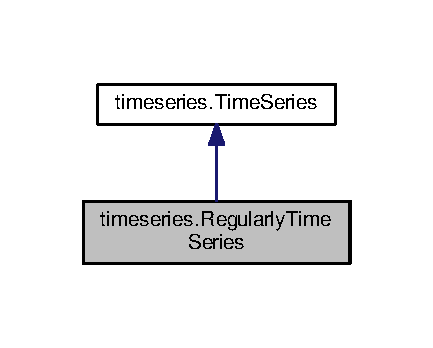
\includegraphics[width=208pt]{classtimeseries_1_1_regularly_time_series__inherit__graph}
\end{center}
\end{figure}


Collaboration diagram for timeseries.\+Regularly\+Time\+Series\+:
\nopagebreak
\begin{figure}[H]
\begin{center}
\leavevmode
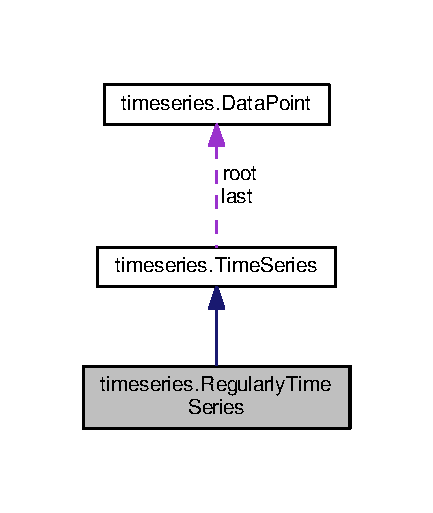
\includegraphics[width=208pt]{classtimeseries_1_1_regularly_time_series__coll__graph}
\end{center}
\end{figure}
\subsection*{Public Member Functions}
\begin{DoxyCompactItemize}
\item 
\hyperlink{classtimeseries_1_1_regularly_time_series_ada900123604958ddae734c40bab636e7}{Regularly\+Time\+Series} ()
\item 
\hyperlink{classtimeseries_1_1_regularly_time_series_a278db93dcce4c470b666d9b5758c838a}{Regularly\+Time\+Series} (double n\+Spacing)
\item 
\hyperlink{classtimeseries_1_1_regularly_time_series_ab02cf758028f6ee2f54cd1b00895348a}{Regularly\+Time\+Series} (double n\+Spacing, double nt, double nx)
\item 
double \hyperlink{classtimeseries_1_1_regularly_time_series_a2cea069690717b0f52775619c5e2aa8e}{get\+Spacing} ()
\item 
long \hyperlink{classtimeseries_1_1_regularly_time_series_a635ace3b88199750c47882d546255515}{size} ()
\item 
void \hyperlink{classtimeseries_1_1_regularly_time_series_a0735eaa4a72c73ea82c65c9691bd2c11}{add\+First\+Data\+Point} (double nt, double nx)
\item 
void \hyperlink{classtimeseries_1_1_regularly_time_series_a81e7fa5652d91d707d99005c8ffef413}{add\+X} (double nx)
\item 
double \hyperlink{classtimeseries_1_1_regularly_time_series_a42fa72dae696838e7ec8842c037bfe6f}{get\+X} (double t)
\item 
\hyperlink{classtimeseries_1_1_regularly_time_series}{Regularly\+Time\+Series} \hyperlink{classtimeseries_1_1_regularly_time_series_a46c28fb21d2fe1adcd9dbf2c3c1f72d2}{sub\+Series} (double ft, double tt)
\item 
\hyperlink{classtimeseries_1_1_regularly_time_series}{Regularly\+Time\+Series} \hyperlink{classtimeseries_1_1_regularly_time_series_a461fceebc34325112ac6f680ccbb78d3}{sub\+Series} (long f\+Index, long t\+Index)
\item 
\hyperlink{classtimeseries_1_1_regularly_time_series}{Regularly\+Time\+Series} \hyperlink{classtimeseries_1_1_regularly_time_series_a4c9c8f659f669b987fa62d95c8820c34}{divert} ()
\end{DoxyCompactItemize}
\subsection*{Additional Inherited Members}


\subsection{Detailed Description}
Created by apolol92 on 20.\+08.\+15. Represents a regulary time series. Regulary time series has got a constant spacing between the data points. The standard spacing in this class is 1. You can change the spacing by the initialization. 

Definition at line 18 of file Regularly\+Time\+Series.\+java.



\subsection{Constructor \& Destructor Documentation}
\hypertarget{classtimeseries_1_1_regularly_time_series_ada900123604958ddae734c40bab636e7}{}\index{timeseries\+::\+Regularly\+Time\+Series@{timeseries\+::\+Regularly\+Time\+Series}!Regularly\+Time\+Series@{Regularly\+Time\+Series}}
\index{Regularly\+Time\+Series@{Regularly\+Time\+Series}!timeseries\+::\+Regularly\+Time\+Series@{timeseries\+::\+Regularly\+Time\+Series}}
\subsubsection[{Regularly\+Time\+Series}]{\setlength{\rightskip}{0pt plus 5cm}timeseries.\+Regularly\+Time\+Series.\+Regularly\+Time\+Series (
\begin{DoxyParamCaption}
{}
\end{DoxyParamCaption}
)}\label{classtimeseries_1_1_regularly_time_series_ada900123604958ddae734c40bab636e7}
Initialize an empty Regularlyt\+Time\+Series with default spacing 1 

Definition at line 28 of file Regularly\+Time\+Series.\+java.

\hypertarget{classtimeseries_1_1_regularly_time_series_a278db93dcce4c470b666d9b5758c838a}{}\index{timeseries\+::\+Regularly\+Time\+Series@{timeseries\+::\+Regularly\+Time\+Series}!Regularly\+Time\+Series@{Regularly\+Time\+Series}}
\index{Regularly\+Time\+Series@{Regularly\+Time\+Series}!timeseries\+::\+Regularly\+Time\+Series@{timeseries\+::\+Regularly\+Time\+Series}}
\subsubsection[{Regularly\+Time\+Series}]{\setlength{\rightskip}{0pt plus 5cm}timeseries.\+Regularly\+Time\+Series.\+Regularly\+Time\+Series (
\begin{DoxyParamCaption}
\item[{double}]{n\+Spacing}
\end{DoxyParamCaption}
)}\label{classtimeseries_1_1_regularly_time_series_a278db93dcce4c470b666d9b5758c838a}
Initialize an empty Regularlyt\+Time\+Series with spacing = n\+Spacing 
\begin{DoxyParams}{Parameters}
{\em n\+Spacing} & specifics the spacing beetween every observation/\+Data\+Point \\
\hline
\end{DoxyParams}


Definition at line 37 of file Regularly\+Time\+Series.\+java.

\hypertarget{classtimeseries_1_1_regularly_time_series_ab02cf758028f6ee2f54cd1b00895348a}{}\index{timeseries\+::\+Regularly\+Time\+Series@{timeseries\+::\+Regularly\+Time\+Series}!Regularly\+Time\+Series@{Regularly\+Time\+Series}}
\index{Regularly\+Time\+Series@{Regularly\+Time\+Series}!timeseries\+::\+Regularly\+Time\+Series@{timeseries\+::\+Regularly\+Time\+Series}}
\subsubsection[{Regularly\+Time\+Series}]{\setlength{\rightskip}{0pt plus 5cm}timeseries.\+Regularly\+Time\+Series.\+Regularly\+Time\+Series (
\begin{DoxyParamCaption}
\item[{double}]{n\+Spacing, }
\item[{double}]{nt, }
\item[{double}]{nx}
\end{DoxyParamCaption}
)}\label{classtimeseries_1_1_regularly_time_series_ab02cf758028f6ee2f54cd1b00895348a}
Initialize a Regulary\+Time\+Series with spacing = n\+Spacing and the first Data\+Point(nt,nx) 
\begin{DoxyParams}{Parameters}
{\em n\+Spacing} & specifics the spacing beetween every observation/\+Data\+Point \\
\hline
{\em nt} & t value(independent value) \\
\hline
{\em nx} & x value(dependent value) \\
\hline
\end{DoxyParams}


Definition at line 48 of file Regularly\+Time\+Series.\+java.



\subsection{Member Function Documentation}
\hypertarget{classtimeseries_1_1_regularly_time_series_a0735eaa4a72c73ea82c65c9691bd2c11}{}\index{timeseries\+::\+Regularly\+Time\+Series@{timeseries\+::\+Regularly\+Time\+Series}!add\+First\+Data\+Point@{add\+First\+Data\+Point}}
\index{add\+First\+Data\+Point@{add\+First\+Data\+Point}!timeseries\+::\+Regularly\+Time\+Series@{timeseries\+::\+Regularly\+Time\+Series}}
\subsubsection[{add\+First\+Data\+Point}]{\setlength{\rightskip}{0pt plus 5cm}void timeseries.\+Regularly\+Time\+Series.\+add\+First\+Data\+Point (
\begin{DoxyParamCaption}
\item[{double}]{nt, }
\item[{double}]{nx}
\end{DoxyParamCaption}
)}\label{classtimeseries_1_1_regularly_time_series_a0735eaa4a72c73ea82c65c9691bd2c11}
If the regularly time series is empty, then use this method to add the first \hyperlink{classtimeseries_1_1_data_point}{Data\+Point}. 
\begin{DoxyParams}{Parameters}
{\em nt} & t-\/value \\
\hline
{\em nx} & x-\/value \\
\hline
\end{DoxyParams}


Definition at line 82 of file Regularly\+Time\+Series.\+java.

\hypertarget{classtimeseries_1_1_regularly_time_series_a81e7fa5652d91d707d99005c8ffef413}{}\index{timeseries\+::\+Regularly\+Time\+Series@{timeseries\+::\+Regularly\+Time\+Series}!add\+X@{add\+X}}
\index{add\+X@{add\+X}!timeseries\+::\+Regularly\+Time\+Series@{timeseries\+::\+Regularly\+Time\+Series}}
\subsubsection[{add\+X}]{\setlength{\rightskip}{0pt plus 5cm}void timeseries.\+Regularly\+Time\+Series.\+add\+X (
\begin{DoxyParamCaption}
\item[{double}]{nx}
\end{DoxyParamCaption}
)}\label{classtimeseries_1_1_regularly_time_series_a81e7fa5652d91d707d99005c8ffef413}
Add a new \hyperlink{classtimeseries_1_1_data_point}{Data\+Point} to the Regularlyt\+Time\+Series. It calculates the t-\/value by itself \& only need the x-\/value. If there was no \hyperlink{classtimeseries_1_1_data_point}{Data\+Point} set till now, it automatically set the \hyperlink{classtimeseries_1_1_data_point}{Data\+Point} t-\/value to 0. 
\begin{DoxyParams}{Parameters}
{\em nx} & x-\/value \\
\hline
\end{DoxyParams}


Definition at line 95 of file Regularly\+Time\+Series.\+java.

\hypertarget{classtimeseries_1_1_regularly_time_series_a4c9c8f659f669b987fa62d95c8820c34}{}\index{timeseries\+::\+Regularly\+Time\+Series@{timeseries\+::\+Regularly\+Time\+Series}!divert@{divert}}
\index{divert@{divert}!timeseries\+::\+Regularly\+Time\+Series@{timeseries\+::\+Regularly\+Time\+Series}}
\subsubsection[{divert}]{\setlength{\rightskip}{0pt plus 5cm}{\bf Regularly\+Time\+Series} timeseries.\+Regularly\+Time\+Series.\+divert (
\begin{DoxyParamCaption}
{}
\end{DoxyParamCaption}
)}\label{classtimeseries_1_1_regularly_time_series_a4c9c8f659f669b987fa62d95c8820c34}
Calculate a diverted time series of the original time series.. It can be used to remove trends from time series.. If you have got a linear trend, divert onetimes.. If you have got a quadratic trend, divert twotimes.. If you have got a n trend, divert n-\/times.. \begin{DoxyReturn}{Returns}
the diverted time series 
\end{DoxyReturn}


Definition at line 193 of file Regularly\+Time\+Series.\+java.

\hypertarget{classtimeseries_1_1_regularly_time_series_a2cea069690717b0f52775619c5e2aa8e}{}\index{timeseries\+::\+Regularly\+Time\+Series@{timeseries\+::\+Regularly\+Time\+Series}!get\+Spacing@{get\+Spacing}}
\index{get\+Spacing@{get\+Spacing}!timeseries\+::\+Regularly\+Time\+Series@{timeseries\+::\+Regularly\+Time\+Series}}
\subsubsection[{get\+Spacing}]{\setlength{\rightskip}{0pt plus 5cm}double timeseries.\+Regularly\+Time\+Series.\+get\+Spacing (
\begin{DoxyParamCaption}
{}
\end{DoxyParamCaption}
)}\label{classtimeseries_1_1_regularly_time_series_a2cea069690717b0f52775619c5e2aa8e}
Gets the spacing between the ticks \begin{DoxyReturn}{Returns}
spacing 
\end{DoxyReturn}


Definition at line 58 of file Regularly\+Time\+Series.\+java.

\hypertarget{classtimeseries_1_1_regularly_time_series_a42fa72dae696838e7ec8842c037bfe6f}{}\index{timeseries\+::\+Regularly\+Time\+Series@{timeseries\+::\+Regularly\+Time\+Series}!get\+X@{get\+X}}
\index{get\+X@{get\+X}!timeseries\+::\+Regularly\+Time\+Series@{timeseries\+::\+Regularly\+Time\+Series}}
\subsubsection[{get\+X}]{\setlength{\rightskip}{0pt plus 5cm}double timeseries.\+Regularly\+Time\+Series.\+get\+X (
\begin{DoxyParamCaption}
\item[{double}]{t}
\end{DoxyParamCaption}
)}\label{classtimeseries_1_1_regularly_time_series_a42fa72dae696838e7ec8842c037bfe6f}
Get the x-\/value at t 
\begin{DoxyParams}{Parameters}
{\em t} & position in time series \\
\hline
\end{DoxyParams}
\begin{DoxyReturn}{Returns}
x-\/value at this position 
\end{DoxyReturn}


Definition at line 110 of file Regularly\+Time\+Series.\+java.

\hypertarget{classtimeseries_1_1_regularly_time_series_a635ace3b88199750c47882d546255515}{}\index{timeseries\+::\+Regularly\+Time\+Series@{timeseries\+::\+Regularly\+Time\+Series}!size@{size}}
\index{size@{size}!timeseries\+::\+Regularly\+Time\+Series@{timeseries\+::\+Regularly\+Time\+Series}}
\subsubsection[{size}]{\setlength{\rightskip}{0pt plus 5cm}long timeseries.\+Regularly\+Time\+Series.\+size (
\begin{DoxyParamCaption}
{}
\end{DoxyParamCaption}
)}\label{classtimeseries_1_1_regularly_time_series_a635ace3b88199750c47882d546255515}
Counts the amount of Data\+Points \begin{DoxyReturn}{Returns}
the amount of Data\+Points 
\end{DoxyReturn}


Definition at line 67 of file Regularly\+Time\+Series.\+java.

\hypertarget{classtimeseries_1_1_regularly_time_series_a46c28fb21d2fe1adcd9dbf2c3c1f72d2}{}\index{timeseries\+::\+Regularly\+Time\+Series@{timeseries\+::\+Regularly\+Time\+Series}!sub\+Series@{sub\+Series}}
\index{sub\+Series@{sub\+Series}!timeseries\+::\+Regularly\+Time\+Series@{timeseries\+::\+Regularly\+Time\+Series}}
\subsubsection[{sub\+Series}]{\setlength{\rightskip}{0pt plus 5cm}{\bf Regularly\+Time\+Series} timeseries.\+Regularly\+Time\+Series.\+sub\+Series (
\begin{DoxyParamCaption}
\item[{double}]{ft, }
\item[{double}]{tt}
\end{DoxyParamCaption}
)}\label{classtimeseries_1_1_regularly_time_series_a46c28fb21d2fe1adcd9dbf2c3c1f72d2}
Creates a sub Regulary\+Time\+Series. 
\begin{DoxyParams}{Parameters}
{\em ft} & from t \\
\hline
{\em tt} & to t (including this one) \\
\hline
\end{DoxyParams}
\begin{DoxyReturn}{Returns}

\end{DoxyReturn}


Definition at line 131 of file Regularly\+Time\+Series.\+java.

\hypertarget{classtimeseries_1_1_regularly_time_series_a461fceebc34325112ac6f680ccbb78d3}{}\index{timeseries\+::\+Regularly\+Time\+Series@{timeseries\+::\+Regularly\+Time\+Series}!sub\+Series@{sub\+Series}}
\index{sub\+Series@{sub\+Series}!timeseries\+::\+Regularly\+Time\+Series@{timeseries\+::\+Regularly\+Time\+Series}}
\subsubsection[{sub\+Series}]{\setlength{\rightskip}{0pt plus 5cm}{\bf Regularly\+Time\+Series} timeseries.\+Regularly\+Time\+Series.\+sub\+Series (
\begin{DoxyParamCaption}
\item[{long}]{f\+Index, }
\item[{long}]{t\+Index}
\end{DoxyParamCaption}
)}\label{classtimeseries_1_1_regularly_time_series_a461fceebc34325112ac6f680ccbb78d3}
Creates a sub Regulary\+Time\+Series 
\begin{DoxyParams}{Parameters}
{\em f\+Index} & from index \\
\hline
{\em t\+Index} & to index (including this one) \\
\hline
\end{DoxyParams}
\begin{DoxyReturn}{Returns}

\end{DoxyReturn}


Definition at line 160 of file Regularly\+Time\+Series.\+java.



The documentation for this class was generated from the following file\+:\begin{DoxyCompactItemize}
\item 
/home/apolol92/\+Dokumente/\+Programmierung/\+Java/\+J\+Time\+Series/src/timeseries/\hyperlink{_regularly_time_series_8java}{Regularly\+Time\+Series.\+java}\end{DoxyCompactItemize}

\hypertarget{classtimeseries_1_1regularly__timeseries_1_1forecasters_1_1exponential__smoothing_1_1_simple_exponential_smoothing}{}\section{timeseries.\+regularly\+\_\+timeseries.\+forecasters.\+exponential\+\_\+smoothing.\+Simple\+Exponential\+Smoothing Class Reference}
\label{classtimeseries_1_1regularly__timeseries_1_1forecasters_1_1exponential__smoothing_1_1_simple_exponential_smoothing}\index{timeseries.\+regularly\+\_\+timeseries.\+forecasters.\+exponential\+\_\+smoothing.\+Simple\+Exponential\+Smoothing@{timeseries.\+regularly\+\_\+timeseries.\+forecasters.\+exponential\+\_\+smoothing.\+Simple\+Exponential\+Smoothing}}
\subsection*{Static Public Member Functions}
\begin{DoxyCompactItemize}
\item 
static \hyperlink{classtimeseries_1_1_regularly_time_series}{Regularly\+Time\+Series} \hyperlink{classtimeseries_1_1regularly__timeseries_1_1forecasters_1_1exponential__smoothing_1_1_simple_exponential_smoothing_afebe870f327de6fa5215edbe4b9c0e3e}{fit} (\hyperlink{classtimeseries_1_1_regularly_time_series}{Regularly\+Time\+Series} ts, double alpha, long h)
\end{DoxyCompactItemize}


\subsection{Detailed Description}
Created by apolol92 on 21.\+08.\+15. Simple exponential smoothing(\+S\+E\+S) uses a weighted moving average with weights that decrease exponentially as observations come from further in the past. S\+E\+S only has a flat forecast function, for longer forecast horizons h $>$= 2, we get\+: y(t+h$\vert$\+T) = y(t+1$\vert$\+T). Disadvantage of S\+E\+S\+: It is only suitable for forecasting data with no trend and no seasonal pattern. 

Definition at line 23 of file Simple\+Exponential\+Smoothing.\+java.



\subsection{Member Function Documentation}
\hypertarget{classtimeseries_1_1regularly__timeseries_1_1forecasters_1_1exponential__smoothing_1_1_simple_exponential_smoothing_afebe870f327de6fa5215edbe4b9c0e3e}{}\index{timeseries\+::regularly\+\_\+timeseries\+::forecasters\+::exponential\+\_\+smoothing\+::\+Simple\+Exponential\+Smoothing@{timeseries\+::regularly\+\_\+timeseries\+::forecasters\+::exponential\+\_\+smoothing\+::\+Simple\+Exponential\+Smoothing}!fit@{fit}}
\index{fit@{fit}!timeseries\+::regularly\+\_\+timeseries\+::forecasters\+::exponential\+\_\+smoothing\+::\+Simple\+Exponential\+Smoothing@{timeseries\+::regularly\+\_\+timeseries\+::forecasters\+::exponential\+\_\+smoothing\+::\+Simple\+Exponential\+Smoothing}}
\subsubsection[{fit}]{\setlength{\rightskip}{0pt plus 5cm}static {\bf Regularly\+Time\+Series} timeseries.\+regularly\+\_\+timeseries.\+forecasters.\+exponential\+\_\+smoothing.\+Simple\+Exponential\+Smoothing.\+fit (
\begin{DoxyParamCaption}
\item[{{\bf Regularly\+Time\+Series}}]{ts, }
\item[{double}]{alpha, }
\item[{long}]{h}
\end{DoxyParamCaption}
)\hspace{0.3cm}{\ttfamily [static]}}\label{classtimeseries_1_1regularly__timeseries_1_1forecasters_1_1exponential__smoothing_1_1_simple_exponential_smoothing_afebe870f327de6fa5215edbe4b9c0e3e}
Creates a time series via S\+E\+S 
\begin{DoxyParams}{Parameters}
{\em ts} & original time series \\
\hline
{\em alpha} & The smoothing parameter alpha with 0 $<$ alpha $<$= 1 controls the weights decrease. \\
\hline
{\em h} & forecasting steps/range \\
\hline
\end{DoxyParams}
\begin{DoxyReturn}{Returns}
simple exponential smoothed time series 
\end{DoxyReturn}


Definition at line 32 of file Simple\+Exponential\+Smoothing.\+java.



The documentation for this class was generated from the following file\+:\begin{DoxyCompactItemize}
\item 
/home/apolol92/\+Dokumente/\+Programmierung/\+Java/\+J\+Time\+Series/src/timeseries/regularly\+\_\+timeseries/forecasters/exponential\+\_\+smoothing/\hyperlink{_simple_exponential_smoothing_8java}{Simple\+Exponential\+Smoothing.\+java}\end{DoxyCompactItemize}

\hypertarget{classtimeseries_1_1regularly__timeseries_1_1forecasters_1_1_simple_forecaster}{}\section{timeseries.\+regularly\+\_\+timeseries.\+forecasters.\+Simple\+Forecaster Class Reference}
\label{classtimeseries_1_1regularly__timeseries_1_1forecasters_1_1_simple_forecaster}\index{timeseries.\+regularly\+\_\+timeseries.\+forecasters.\+Simple\+Forecaster@{timeseries.\+regularly\+\_\+timeseries.\+forecasters.\+Simple\+Forecaster}}
\subsection*{Static Public Member Functions}
\begin{DoxyCompactItemize}
\item 
static double \hyperlink{classtimeseries_1_1regularly__timeseries_1_1forecasters_1_1_simple_forecaster_a84564c513ad7970d9cc1b6619b462023}{average\+Method} (\hyperlink{classtimeseries_1_1_regularly_time_series}{Regularly\+Time\+Series} ts)
\item 
static double \hyperlink{classtimeseries_1_1regularly__timeseries_1_1forecasters_1_1_simple_forecaster_aff68d3d40969d8564dc5c0c60b4df361}{naive\+\_\+method} (\hyperlink{classtimeseries_1_1_regularly_time_series}{Regularly\+Time\+Series} ts)
\end{DoxyCompactItemize}


\subsection{Detailed Description}
Created by apolol92 on 21.\+08.\+15. This class offers static methods for simple forecasting.. 

Definition at line 18 of file Simple\+Forecaster.\+java.



\subsection{Member Function Documentation}
\hypertarget{classtimeseries_1_1regularly__timeseries_1_1forecasters_1_1_simple_forecaster_a84564c513ad7970d9cc1b6619b462023}{}\index{timeseries\+::regularly\+\_\+timeseries\+::forecasters\+::\+Simple\+Forecaster@{timeseries\+::regularly\+\_\+timeseries\+::forecasters\+::\+Simple\+Forecaster}!average\+Method@{average\+Method}}
\index{average\+Method@{average\+Method}!timeseries\+::regularly\+\_\+timeseries\+::forecasters\+::\+Simple\+Forecaster@{timeseries\+::regularly\+\_\+timeseries\+::forecasters\+::\+Simple\+Forecaster}}
\subsubsection[{average\+Method}]{\setlength{\rightskip}{0pt plus 5cm}static double timeseries.\+regularly\+\_\+timeseries.\+forecasters.\+Simple\+Forecaster.\+average\+Method (
\begin{DoxyParamCaption}
\item[{{\bf Regularly\+Time\+Series}}]{ts}
\end{DoxyParamCaption}
)\hspace{0.3cm}{\ttfamily [static]}}\label{classtimeseries_1_1regularly__timeseries_1_1forecasters_1_1_simple_forecaster_a84564c513ad7970d9cc1b6619b462023}
mean value of historical data 
\begin{DoxyParams}{Parameters}
{\em ts,historical} & data \\
\hline
\end{DoxyParams}
\begin{DoxyReturn}{Returns}
forecast 
\end{DoxyReturn}


Definition at line 25 of file Simple\+Forecaster.\+java.

\hypertarget{classtimeseries_1_1regularly__timeseries_1_1forecasters_1_1_simple_forecaster_aff68d3d40969d8564dc5c0c60b4df361}{}\index{timeseries\+::regularly\+\_\+timeseries\+::forecasters\+::\+Simple\+Forecaster@{timeseries\+::regularly\+\_\+timeseries\+::forecasters\+::\+Simple\+Forecaster}!naive\+\_\+method@{naive\+\_\+method}}
\index{naive\+\_\+method@{naive\+\_\+method}!timeseries\+::regularly\+\_\+timeseries\+::forecasters\+::\+Simple\+Forecaster@{timeseries\+::regularly\+\_\+timeseries\+::forecasters\+::\+Simple\+Forecaster}}
\subsubsection[{naive\+\_\+method}]{\setlength{\rightskip}{0pt plus 5cm}static double timeseries.\+regularly\+\_\+timeseries.\+forecasters.\+Simple\+Forecaster.\+naive\+\_\+method (
\begin{DoxyParamCaption}
\item[{{\bf Regularly\+Time\+Series}}]{ts}
\end{DoxyParamCaption}
)\hspace{0.3cm}{\ttfamily [static]}}\label{classtimeseries_1_1regularly__timeseries_1_1forecasters_1_1_simple_forecaster_aff68d3d40969d8564dc5c0c60b4df361}
last observed value 
\begin{DoxyParams}{Parameters}
{\em ts,historical} & data \\
\hline
\end{DoxyParams}
\begin{DoxyReturn}{Returns}
forecast 
\end{DoxyReturn}


Definition at line 34 of file Simple\+Forecaster.\+java.



The documentation for this class was generated from the following file\+:\begin{DoxyCompactItemize}
\item 
/home/apolol92/\+Dokumente/\+Programmierung/\+Java/\+J\+Time\+Series/src/timeseries/regularly\+\_\+timeseries/forecasters/\hyperlink{_simple_forecaster_8java}{Simple\+Forecaster.\+java}\end{DoxyCompactItemize}

\hypertarget{classtimeseries_1_1_time_series}{}\section{timeseries.\+Time\+Series Class Reference}
\label{classtimeseries_1_1_time_series}\index{timeseries.\+Time\+Series@{timeseries.\+Time\+Series}}


Inheritance diagram for timeseries.\+Time\+Series\+:
\nopagebreak
\begin{figure}[H]
\begin{center}
\leavevmode
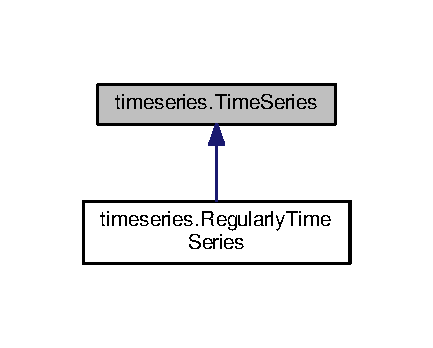
\includegraphics[width=208pt]{classtimeseries_1_1_time_series__inherit__graph}
\end{center}
\end{figure}


Collaboration diagram for timeseries.\+Time\+Series\+:
\nopagebreak
\begin{figure}[H]
\begin{center}
\leavevmode
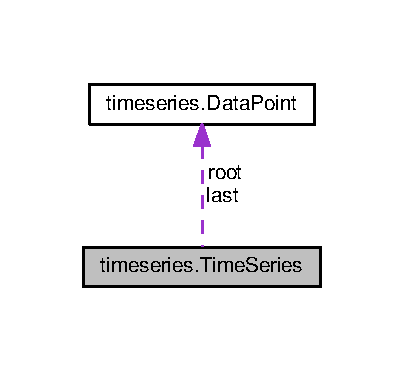
\includegraphics[width=194pt]{classtimeseries_1_1_time_series__coll__graph}
\end{center}
\end{figure}
\subsection*{Public Member Functions}
\begin{DoxyCompactItemize}
\item 
abstract long \hyperlink{classtimeseries_1_1_time_series_a390324a52568f45892838f08142b8e44}{size} ()
\item 
double \hyperlink{classtimeseries_1_1_time_series_a21a48f6a58aefd8b7261acccfc442425}{length} ()
\item 
double \hyperlink{classtimeseries_1_1_time_series_a756d884d57220f887a2425e850450f33}{get\+T} (long index)
\item 
double \hyperlink{classtimeseries_1_1_time_series_a1bf3cb62b9976193264b68ef8d001919}{get\+X} (long index)
\item 
double \hyperlink{classtimeseries_1_1_time_series_a0cd53da9484fd4ee3b5c5110e79c0a7e}{get\+Gradient} (long index)
\item 
double \hyperlink{classtimeseries_1_1_time_series_ac841bb482c0ef9fe79839c255406c8c6}{max} ()
\item 
double \hyperlink{classtimeseries_1_1_time_series_a06f25367736b3f59807e6f060650bc7e}{min} ()
\item 
double \hyperlink{classtimeseries_1_1_time_series_a70d9b8388e8b729ce9a719b25d3016aa}{mean} ()
\item 
double \hyperlink{classtimeseries_1_1_time_series_a255d92682fb235b5c9dbb4d803d7f8d3}{variance} ()
\item 
double \hyperlink{classtimeseries_1_1_time_series_a326e8450cc7ce9bc2118255227d20664}{standard\+Deviation} ()
\item 
double \hyperlink{classtimeseries_1_1_time_series_a7851e2236b47e0c3440a949bda2bea91}{median} ()
\item 
abstract \hyperlink{classtimeseries_1_1_time_series}{Time\+Series} \hyperlink{classtimeseries_1_1_time_series_ac3422314d9131982a0c8f35eb4a99fc2}{sub\+Series} (double ft, double tt)
\item 
abstract \hyperlink{classtimeseries_1_1_time_series}{Time\+Series} \hyperlink{classtimeseries_1_1_time_series_a13599863c16f9c8c029c1f0ba9a17202}{sub\+Series} (long f\+Index, long t\+Index)
\item 
abstract \hyperlink{classtimeseries_1_1_time_series}{Time\+Series} \hyperlink{classtimeseries_1_1_time_series_a91f886289adc77eb25bb5f58667d2049}{divert} ()
\item 
String \hyperlink{classtimeseries_1_1_time_series_abc1e7b0fb89081f2214c7ef29efe23b2}{to\+String} ()
\end{DoxyCompactItemize}
\subsection*{Protected Member Functions}
\begin{DoxyCompactItemize}
\item 
\hyperlink{classtimeseries_1_1_time_series_ace12d3eb25b3d267b90c7c08a4f4445d}{Time\+Series} ()
\end{DoxyCompactItemize}
\subsection*{Protected Attributes}
\begin{DoxyCompactItemize}
\item 
\hyperlink{classtimeseries_1_1_data_point}{Data\+Point} \hyperlink{classtimeseries_1_1_time_series_affc228300a6e7aeff7646df39da9269a}{root}
\item 
\hyperlink{classtimeseries_1_1_data_point}{Data\+Point} \hyperlink{classtimeseries_1_1_time_series_afeb87d5f2b84516c9cad5623a497a783}{last}
\end{DoxyCompactItemize}


\subsection{Detailed Description}
Created by apolol92 on 20.\+08.\+15. Represents a time series. A time series is a sequence of data points. There are two types of time series\+:
\begin{DoxyItemize}
\item Regular time series\+: The spacing between every observation/data point is always the same
\item Irregular time series\+: The spacing between every observation/data point is different But these two types have much in common. For this reason we use an abstract parent class called \hyperlink{classtimeseries_1_1_time_series}{Time\+Series}. 
\end{DoxyItemize}

Definition at line 23 of file Time\+Series.\+java.



\subsection{Constructor \& Destructor Documentation}
\hypertarget{classtimeseries_1_1_time_series_ace12d3eb25b3d267b90c7c08a4f4445d}{}\index{timeseries\+::\+Time\+Series@{timeseries\+::\+Time\+Series}!Time\+Series@{Time\+Series}}
\index{Time\+Series@{Time\+Series}!timeseries\+::\+Time\+Series@{timeseries\+::\+Time\+Series}}
\subsubsection[{Time\+Series}]{\setlength{\rightskip}{0pt plus 5cm}timeseries.\+Time\+Series.\+Time\+Series (
\begin{DoxyParamCaption}
{}
\end{DoxyParamCaption}
)\hspace{0.3cm}{\ttfamily [protected]}}\label{classtimeseries_1_1_time_series_ace12d3eb25b3d267b90c7c08a4f4445d}
This standard constructor initialize the \hyperlink{classtimeseries_1_1_time_series}{Time\+Series}. 

Definition at line 37 of file Time\+Series.\+java.



\subsection{Member Function Documentation}
\hypertarget{classtimeseries_1_1_time_series_a91f886289adc77eb25bb5f58667d2049}{}\index{timeseries\+::\+Time\+Series@{timeseries\+::\+Time\+Series}!divert@{divert}}
\index{divert@{divert}!timeseries\+::\+Time\+Series@{timeseries\+::\+Time\+Series}}
\subsubsection[{divert}]{\setlength{\rightskip}{0pt plus 5cm}abstract {\bf Time\+Series} timeseries.\+Time\+Series.\+divert (
\begin{DoxyParamCaption}
{}
\end{DoxyParamCaption}
)\hspace{0.3cm}{\ttfamily [abstract]}}\label{classtimeseries_1_1_time_series_a91f886289adc77eb25bb5f58667d2049}
This method will divert the time series.. \begin{DoxyReturn}{Returns}
the diverted time series.. 
\end{DoxyReturn}
\hypertarget{classtimeseries_1_1_time_series_a0cd53da9484fd4ee3b5c5110e79c0a7e}{}\index{timeseries\+::\+Time\+Series@{timeseries\+::\+Time\+Series}!get\+Gradient@{get\+Gradient}}
\index{get\+Gradient@{get\+Gradient}!timeseries\+::\+Time\+Series@{timeseries\+::\+Time\+Series}}
\subsubsection[{get\+Gradient}]{\setlength{\rightskip}{0pt plus 5cm}double timeseries.\+Time\+Series.\+get\+Gradient (
\begin{DoxyParamCaption}
\item[{long}]{index}
\end{DoxyParamCaption}
)}\label{classtimeseries_1_1_time_series_a0cd53da9484fd4ee3b5c5110e79c0a7e}
Gets the x value of a \hyperlink{classtimeseries_1_1_data_point}{Data\+Point} at index position \char`\"{}index\char`\"{}. 

Definition at line 94 of file Time\+Series.\+java.

\hypertarget{classtimeseries_1_1_time_series_a756d884d57220f887a2425e850450f33}{}\index{timeseries\+::\+Time\+Series@{timeseries\+::\+Time\+Series}!get\+T@{get\+T}}
\index{get\+T@{get\+T}!timeseries\+::\+Time\+Series@{timeseries\+::\+Time\+Series}}
\subsubsection[{get\+T}]{\setlength{\rightskip}{0pt plus 5cm}double timeseries.\+Time\+Series.\+get\+T (
\begin{DoxyParamCaption}
\item[{long}]{index}
\end{DoxyParamCaption}
)}\label{classtimeseries_1_1_time_series_a756d884d57220f887a2425e850450f33}
Gets the t-\/value at index \char`\"{}index\char`\"{} 
\begin{DoxyParams}{Parameters}
{\em index} & \\
\hline
\end{DoxyParams}
\begin{DoxyReturn}{Returns}
t-\/value 
\end{DoxyReturn}


Definition at line 62 of file Time\+Series.\+java.

\hypertarget{classtimeseries_1_1_time_series_a1bf3cb62b9976193264b68ef8d001919}{}\index{timeseries\+::\+Time\+Series@{timeseries\+::\+Time\+Series}!get\+X@{get\+X}}
\index{get\+X@{get\+X}!timeseries\+::\+Time\+Series@{timeseries\+::\+Time\+Series}}
\subsubsection[{get\+X}]{\setlength{\rightskip}{0pt plus 5cm}double timeseries.\+Time\+Series.\+get\+X (
\begin{DoxyParamCaption}
\item[{long}]{index}
\end{DoxyParamCaption}
)}\label{classtimeseries_1_1_time_series_a1bf3cb62b9976193264b68ef8d001919}
Gets the x value of a \hyperlink{classtimeseries_1_1_data_point}{Data\+Point} at index position \char`\"{}index\char`\"{}. 

Definition at line 78 of file Time\+Series.\+java.

\hypertarget{classtimeseries_1_1_time_series_a21a48f6a58aefd8b7261acccfc442425}{}\index{timeseries\+::\+Time\+Series@{timeseries\+::\+Time\+Series}!length@{length}}
\index{length@{length}!timeseries\+::\+Time\+Series@{timeseries\+::\+Time\+Series}}
\subsubsection[{length}]{\setlength{\rightskip}{0pt plus 5cm}double timeseries.\+Time\+Series.\+length (
\begin{DoxyParamCaption}
{}
\end{DoxyParamCaption}
)}\label{classtimeseries_1_1_time_series_a21a48f6a58aefd8b7261acccfc442425}
This method measures the length of the \hyperlink{classtimeseries_1_1_time_series}{Time\+Series}. Distance between the root \hyperlink{classtimeseries_1_1_data_point}{Data\+Point} and the last \hyperlink{classtimeseries_1_1_data_point}{Data\+Point} \begin{DoxyReturn}{Returns}

\end{DoxyReturn}


Definition at line 53 of file Time\+Series.\+java.

\hypertarget{classtimeseries_1_1_time_series_ac841bb482c0ef9fe79839c255406c8c6}{}\index{timeseries\+::\+Time\+Series@{timeseries\+::\+Time\+Series}!max@{max}}
\index{max@{max}!timeseries\+::\+Time\+Series@{timeseries\+::\+Time\+Series}}
\subsubsection[{max}]{\setlength{\rightskip}{0pt plus 5cm}double timeseries.\+Time\+Series.\+max (
\begin{DoxyParamCaption}
{}
\end{DoxyParamCaption}
)}\label{classtimeseries_1_1_time_series_ac841bb482c0ef9fe79839c255406c8c6}
Calculates the max value of the time series \begin{DoxyReturn}{Returns}
the max value 
\end{DoxyReturn}


Definition at line 112 of file Time\+Series.\+java.

\hypertarget{classtimeseries_1_1_time_series_a70d9b8388e8b729ce9a719b25d3016aa}{}\index{timeseries\+::\+Time\+Series@{timeseries\+::\+Time\+Series}!mean@{mean}}
\index{mean@{mean}!timeseries\+::\+Time\+Series@{timeseries\+::\+Time\+Series}}
\subsubsection[{mean}]{\setlength{\rightskip}{0pt plus 5cm}double timeseries.\+Time\+Series.\+mean (
\begin{DoxyParamCaption}
{}
\end{DoxyParamCaption}
)}\label{classtimeseries_1_1_time_series_a70d9b8388e8b729ce9a719b25d3016aa}
Calculates the mean value of the time series \begin{DoxyReturn}{Returns}

\end{DoxyReturn}


Definition at line 144 of file Time\+Series.\+java.

\hypertarget{classtimeseries_1_1_time_series_a7851e2236b47e0c3440a949bda2bea91}{}\index{timeseries\+::\+Time\+Series@{timeseries\+::\+Time\+Series}!median@{median}}
\index{median@{median}!timeseries\+::\+Time\+Series@{timeseries\+::\+Time\+Series}}
\subsubsection[{median}]{\setlength{\rightskip}{0pt plus 5cm}double timeseries.\+Time\+Series.\+median (
\begin{DoxyParamCaption}
{}
\end{DoxyParamCaption}
)}\label{classtimeseries_1_1_time_series_a7851e2236b47e0c3440a949bda2bea91}
Calculates the median of the time series \begin{DoxyReturn}{Returns}
the median 
\end{DoxyReturn}


Definition at line 185 of file Time\+Series.\+java.

\hypertarget{classtimeseries_1_1_time_series_a06f25367736b3f59807e6f060650bc7e}{}\index{timeseries\+::\+Time\+Series@{timeseries\+::\+Time\+Series}!min@{min}}
\index{min@{min}!timeseries\+::\+Time\+Series@{timeseries\+::\+Time\+Series}}
\subsubsection[{min}]{\setlength{\rightskip}{0pt plus 5cm}double timeseries.\+Time\+Series.\+min (
\begin{DoxyParamCaption}
{}
\end{DoxyParamCaption}
)}\label{classtimeseries_1_1_time_series_a06f25367736b3f59807e6f060650bc7e}
Calculates the min value of the time series \begin{DoxyReturn}{Returns}
the min value 
\end{DoxyReturn}


Definition at line 128 of file Time\+Series.\+java.

\hypertarget{classtimeseries_1_1_time_series_a390324a52568f45892838f08142b8e44}{}\index{timeseries\+::\+Time\+Series@{timeseries\+::\+Time\+Series}!size@{size}}
\index{size@{size}!timeseries\+::\+Time\+Series@{timeseries\+::\+Time\+Series}}
\subsubsection[{size}]{\setlength{\rightskip}{0pt plus 5cm}abstract long timeseries.\+Time\+Series.\+size (
\begin{DoxyParamCaption}
{}
\end{DoxyParamCaption}
)\hspace{0.3cm}{\ttfamily [abstract]}}\label{classtimeseries_1_1_time_series_a390324a52568f45892838f08142b8e44}
This method counts the Data\+Points in the \hyperlink{classtimeseries_1_1_time_series}{Time\+Series}. \begin{DoxyReturn}{Returns}
amount of Data\+Points 
\end{DoxyReturn}
\hypertarget{classtimeseries_1_1_time_series_a326e8450cc7ce9bc2118255227d20664}{}\index{timeseries\+::\+Time\+Series@{timeseries\+::\+Time\+Series}!standard\+Deviation@{standard\+Deviation}}
\index{standard\+Deviation@{standard\+Deviation}!timeseries\+::\+Time\+Series@{timeseries\+::\+Time\+Series}}
\subsubsection[{standard\+Deviation}]{\setlength{\rightskip}{0pt plus 5cm}double timeseries.\+Time\+Series.\+standard\+Deviation (
\begin{DoxyParamCaption}
{}
\end{DoxyParamCaption}
)}\label{classtimeseries_1_1_time_series_a326e8450cc7ce9bc2118255227d20664}
Calculates the standard deviaton of the time series \begin{DoxyReturn}{Returns}
the standard deviation 
\end{DoxyReturn}


Definition at line 177 of file Time\+Series.\+java.

\hypertarget{classtimeseries_1_1_time_series_ac3422314d9131982a0c8f35eb4a99fc2}{}\index{timeseries\+::\+Time\+Series@{timeseries\+::\+Time\+Series}!sub\+Series@{sub\+Series}}
\index{sub\+Series@{sub\+Series}!timeseries\+::\+Time\+Series@{timeseries\+::\+Time\+Series}}
\subsubsection[{sub\+Series}]{\setlength{\rightskip}{0pt plus 5cm}abstract {\bf Time\+Series} timeseries.\+Time\+Series.\+sub\+Series (
\begin{DoxyParamCaption}
\item[{double}]{ft, }
\item[{double}]{tt}
\end{DoxyParamCaption}
)\hspace{0.3cm}{\ttfamily [abstract]}}\label{classtimeseries_1_1_time_series_ac3422314d9131982a0c8f35eb4a99fc2}
Will create a sub time series of the current one. This sub time series is totally independent from his parent 
\begin{DoxyParams}{Parameters}
{\em ft} & from t \\
\hline
{\em tt} & to t (including this one) \\
\hline
\end{DoxyParams}
\begin{DoxyReturn}{Returns}
a time series from t to t 
\end{DoxyReturn}
\hypertarget{classtimeseries_1_1_time_series_a13599863c16f9c8c029c1f0ba9a17202}{}\index{timeseries\+::\+Time\+Series@{timeseries\+::\+Time\+Series}!sub\+Series@{sub\+Series}}
\index{sub\+Series@{sub\+Series}!timeseries\+::\+Time\+Series@{timeseries\+::\+Time\+Series}}
\subsubsection[{sub\+Series}]{\setlength{\rightskip}{0pt plus 5cm}abstract {\bf Time\+Series} timeseries.\+Time\+Series.\+sub\+Series (
\begin{DoxyParamCaption}
\item[{long}]{f\+Index, }
\item[{long}]{t\+Index}
\end{DoxyParamCaption}
)\hspace{0.3cm}{\ttfamily [abstract]}}\label{classtimeseries_1_1_time_series_a13599863c16f9c8c029c1f0ba9a17202}
Will create a sub time series of the current one. This sub time series is totally independent from his parent 
\begin{DoxyParams}{Parameters}
{\em f\+Index} & from index \\
\hline
{\em t\+Index} & to index (including this one) \\
\hline
\end{DoxyParams}
\begin{DoxyReturn}{Returns}
a time series from index to index 
\end{DoxyReturn}
\hypertarget{classtimeseries_1_1_time_series_abc1e7b0fb89081f2214c7ef29efe23b2}{}\index{timeseries\+::\+Time\+Series@{timeseries\+::\+Time\+Series}!to\+String@{to\+String}}
\index{to\+String@{to\+String}!timeseries\+::\+Time\+Series@{timeseries\+::\+Time\+Series}}
\subsubsection[{to\+String}]{\setlength{\rightskip}{0pt plus 5cm}String timeseries.\+Time\+Series.\+to\+String (
\begin{DoxyParamCaption}
{}
\end{DoxyParamCaption}
)}\label{classtimeseries_1_1_time_series_abc1e7b0fb89081f2214c7ef29efe23b2}


Definition at line 214 of file Time\+Series.\+java.

\hypertarget{classtimeseries_1_1_time_series_a255d92682fb235b5c9dbb4d803d7f8d3}{}\index{timeseries\+::\+Time\+Series@{timeseries\+::\+Time\+Series}!variance@{variance}}
\index{variance@{variance}!timeseries\+::\+Time\+Series@{timeseries\+::\+Time\+Series}}
\subsubsection[{variance}]{\setlength{\rightskip}{0pt plus 5cm}double timeseries.\+Time\+Series.\+variance (
\begin{DoxyParamCaption}
{}
\end{DoxyParamCaption}
)}\label{classtimeseries_1_1_time_series_a255d92682fb235b5c9dbb4d803d7f8d3}
Calculates the variance of the time series \begin{DoxyReturn}{Returns}
the variance 
\end{DoxyReturn}


Definition at line 163 of file Time\+Series.\+java.



\subsection{Member Data Documentation}
\hypertarget{classtimeseries_1_1_time_series_afeb87d5f2b84516c9cad5623a497a783}{}\index{timeseries\+::\+Time\+Series@{timeseries\+::\+Time\+Series}!last@{last}}
\index{last@{last}!timeseries\+::\+Time\+Series@{timeseries\+::\+Time\+Series}}
\subsubsection[{last}]{\setlength{\rightskip}{0pt plus 5cm}{\bf Data\+Point} timeseries.\+Time\+Series.\+last\hspace{0.3cm}{\ttfamily [protected]}}\label{classtimeseries_1_1_time_series_afeb87d5f2b84516c9cad5623a497a783}
This is a reference on the latest \hyperlink{classtimeseries_1_1_data_point}{Data\+Point} of the time series. This reference often changes. 

Definition at line 32 of file Time\+Series.\+java.

\hypertarget{classtimeseries_1_1_time_series_affc228300a6e7aeff7646df39da9269a}{}\index{timeseries\+::\+Time\+Series@{timeseries\+::\+Time\+Series}!root@{root}}
\index{root@{root}!timeseries\+::\+Time\+Series@{timeseries\+::\+Time\+Series}}
\subsubsection[{root}]{\setlength{\rightskip}{0pt plus 5cm}{\bf Data\+Point} timeseries.\+Time\+Series.\+root\hspace{0.3cm}{\ttfamily [protected]}}\label{classtimeseries_1_1_time_series_affc228300a6e7aeff7646df39da9269a}
This is a reference on the root \hyperlink{classtimeseries_1_1_data_point}{Data\+Point} of the time series 

Definition at line 27 of file Time\+Series.\+java.



The documentation for this class was generated from the following file\+:\begin{DoxyCompactItemize}
\item 
/home/apolol92/\+Dokumente/\+Programmierung/\+Java/\+J\+Time\+Series/src/timeseries/\hyperlink{_time_series_8java}{Time\+Series.\+java}\end{DoxyCompactItemize}

\chapter{File Documentation}
\hypertarget{_program_8java}{}\section{/home/apolol92/\+Dokumente/\+Programmierung/\+Java/\+J\+Time\+Series/src/main/\+Program.java File Reference}
\label{_program_8java}\index{/home/apolol92/\+Dokumente/\+Programmierung/\+Java/\+J\+Time\+Series/src/main/\+Program.\+java@{/home/apolol92/\+Dokumente/\+Programmierung/\+Java/\+J\+Time\+Series/src/main/\+Program.\+java}}
\subsection*{Classes}
\begin{DoxyCompactItemize}
\item 
class \hyperlink{classmain_1_1_program}{main.\+Program}
\end{DoxyCompactItemize}
\subsection*{Packages}
\begin{DoxyCompactItemize}
\item 
package \hyperlink{namespacemain}{main}
\end{DoxyCompactItemize}

\hypertarget{_data_point_8java}{}\section{/home/apolol92/\+Dokumente/\+Programmierung/\+Java/\+J\+Time\+Series/src/timeseries/\+Data\+Point.java File Reference}
\label{_data_point_8java}\index{/home/apolol92/\+Dokumente/\+Programmierung/\+Java/\+J\+Time\+Series/src/timeseries/\+Data\+Point.\+java@{/home/apolol92/\+Dokumente/\+Programmierung/\+Java/\+J\+Time\+Series/src/timeseries/\+Data\+Point.\+java}}
\subsection*{Classes}
\begin{DoxyCompactItemize}
\item 
class \hyperlink{classtimeseries_1_1_data_point}{timeseries.\+Data\+Point}
\end{DoxyCompactItemize}
\subsection*{Packages}
\begin{DoxyCompactItemize}
\item 
package \hyperlink{namespacetimeseries}{timeseries}
\end{DoxyCompactItemize}

\hypertarget{_evaluator_8java}{}\section{/home/apolol92/\+Dokumente/\+Programmierung/\+Java/\+J\+Time\+Series/src/timeseries/regularly\+\_\+timeseries/evaluation/\+Evaluator.java File Reference}
\label{_evaluator_8java}\index{/home/apolol92/\+Dokumente/\+Programmierung/\+Java/\+J\+Time\+Series/src/timeseries/regularly\+\_\+timeseries/evaluation/\+Evaluator.\+java@{/home/apolol92/\+Dokumente/\+Programmierung/\+Java/\+J\+Time\+Series/src/timeseries/regularly\+\_\+timeseries/evaluation/\+Evaluator.\+java}}
\subsection*{Classes}
\begin{DoxyCompactItemize}
\item 
class \hyperlink{classtimeseries_1_1regularly__timeseries_1_1evaluation_1_1_evaluator}{timeseries.\+regularly\+\_\+timeseries.\+evaluation.\+Evaluator}
\end{DoxyCompactItemize}
\subsection*{Packages}
\begin{DoxyCompactItemize}
\item 
package \hyperlink{namespacetimeseries_1_1regularly__timeseries_1_1evaluation}{timeseries.\+regularly\+\_\+timeseries.\+evaluation}
\end{DoxyCompactItemize}

\hypertarget{_moving_average_filter_8java}{}\section{/home/apolol92/\+Dokumente/\+Programmierung/\+Java/\+J\+Time\+Series/src/timeseries/regularly\+\_\+timeseries/filter/\+Moving\+Average\+Filter.java File Reference}
\label{_moving_average_filter_8java}\index{/home/apolol92/\+Dokumente/\+Programmierung/\+Java/\+J\+Time\+Series/src/timeseries/regularly\+\_\+timeseries/filter/\+Moving\+Average\+Filter.\+java@{/home/apolol92/\+Dokumente/\+Programmierung/\+Java/\+J\+Time\+Series/src/timeseries/regularly\+\_\+timeseries/filter/\+Moving\+Average\+Filter.\+java}}
\subsection*{Classes}
\begin{DoxyCompactItemize}
\item 
class \hyperlink{classtimeseries_1_1regularly__timeseries_1_1filter_1_1_moving_average_filter}{timeseries.\+regularly\+\_\+timeseries.\+filter.\+Moving\+Average\+Filter}
\end{DoxyCompactItemize}
\subsection*{Packages}
\begin{DoxyCompactItemize}
\item 
package \hyperlink{namespacetimeseries_1_1regularly__timeseries_1_1filter}{timeseries.\+regularly\+\_\+timeseries.\+filter}
\end{DoxyCompactItemize}

\hypertarget{_damped_trend_method_8java}{}\section{/home/apolol92/\+Dokumente/\+Programmierung/\+Java/\+J\+Time\+Series/src/timeseries/regularly\+\_\+timeseries/forecasters/exponential\+\_\+smoothing/\+Damped\+Trend\+Method.java File Reference}
\label{_damped_trend_method_8java}\index{/home/apolol92/\+Dokumente/\+Programmierung/\+Java/\+J\+Time\+Series/src/timeseries/regularly\+\_\+timeseries/forecasters/exponential\+\_\+smoothing/\+Damped\+Trend\+Method.\+java@{/home/apolol92/\+Dokumente/\+Programmierung/\+Java/\+J\+Time\+Series/src/timeseries/regularly\+\_\+timeseries/forecasters/exponential\+\_\+smoothing/\+Damped\+Trend\+Method.\+java}}
\subsection*{Classes}
\begin{DoxyCompactItemize}
\item 
class \hyperlink{classtimeseries_1_1regularly__timeseries_1_1forecasters_1_1exponential__smoothing_1_1_damped_trend_method}{timeseries.\+regularly\+\_\+timeseries.\+forecasters.\+exponential\+\_\+smoothing.\+Damped\+Trend\+Method}
\end{DoxyCompactItemize}
\subsection*{Packages}
\begin{DoxyCompactItemize}
\item 
package \hyperlink{namespacetimeseries_1_1regularly__timeseries_1_1forecasters_1_1exponential__smoothing}{timeseries.\+regularly\+\_\+timeseries.\+forecasters.\+exponential\+\_\+smoothing}
\end{DoxyCompactItemize}

\hypertarget{_exponential_trend_method_8java}{}\section{/home/apolol92/\+Dokumente/\+Programmierung/\+Java/\+J\+Time\+Series/src/timeseries/regularly\+\_\+timeseries/forecasters/exponential\+\_\+smoothing/\+Exponential\+Trend\+Method.java File Reference}
\label{_exponential_trend_method_8java}\index{/home/apolol92/\+Dokumente/\+Programmierung/\+Java/\+J\+Time\+Series/src/timeseries/regularly\+\_\+timeseries/forecasters/exponential\+\_\+smoothing/\+Exponential\+Trend\+Method.\+java@{/home/apolol92/\+Dokumente/\+Programmierung/\+Java/\+J\+Time\+Series/src/timeseries/regularly\+\_\+timeseries/forecasters/exponential\+\_\+smoothing/\+Exponential\+Trend\+Method.\+java}}
\subsection*{Classes}
\begin{DoxyCompactItemize}
\item 
class \hyperlink{classtimeseries_1_1regularly__timeseries_1_1forecasters_1_1exponential__smoothing_1_1_exponential_trend_method}{timeseries.\+regularly\+\_\+timeseries.\+forecasters.\+exponential\+\_\+smoothing.\+Exponential\+Trend\+Method}
\end{DoxyCompactItemize}
\subsection*{Packages}
\begin{DoxyCompactItemize}
\item 
package \hyperlink{namespacetimeseries_1_1regularly__timeseries_1_1forecasters_1_1exponential__smoothing}{timeseries.\+regularly\+\_\+timeseries.\+forecasters.\+exponential\+\_\+smoothing}
\end{DoxyCompactItemize}

\hypertarget{_holts_linear_trend_method_8java}{}\section{/home/apolol92/\+Dokumente/\+Programmierung/\+Java/\+J\+Time\+Series/src/timeseries/regularly\+\_\+timeseries/forecasters/exponential\+\_\+smoothing/\+Holts\+Linear\+Trend\+Method.java File Reference}
\label{_holts_linear_trend_method_8java}\index{/home/apolol92/\+Dokumente/\+Programmierung/\+Java/\+J\+Time\+Series/src/timeseries/regularly\+\_\+timeseries/forecasters/exponential\+\_\+smoothing/\+Holts\+Linear\+Trend\+Method.\+java@{/home/apolol92/\+Dokumente/\+Programmierung/\+Java/\+J\+Time\+Series/src/timeseries/regularly\+\_\+timeseries/forecasters/exponential\+\_\+smoothing/\+Holts\+Linear\+Trend\+Method.\+java}}
\subsection*{Classes}
\begin{DoxyCompactItemize}
\item 
class \hyperlink{classtimeseries_1_1regularly__timeseries_1_1forecasters_1_1exponential__smoothing_1_1_holts_linear_trend_method}{timeseries.\+regularly\+\_\+timeseries.\+forecasters.\+exponential\+\_\+smoothing.\+Holts\+Linear\+Trend\+Method}
\end{DoxyCompactItemize}
\subsection*{Packages}
\begin{DoxyCompactItemize}
\item 
package \hyperlink{namespacetimeseries_1_1regularly__timeseries_1_1forecasters_1_1exponential__smoothing}{timeseries.\+regularly\+\_\+timeseries.\+forecasters.\+exponential\+\_\+smoothing}
\end{DoxyCompactItemize}

\hypertarget{_multiplicative_damped_trend_8java}{}\section{/home/apolol92/\+Dokumente/\+Programmierung/\+Java/\+J\+Time\+Series/src/timeseries/regularly\+\_\+timeseries/forecasters/exponential\+\_\+smoothing/\+Multiplicative\+Damped\+Trend.java File Reference}
\label{_multiplicative_damped_trend_8java}\index{/home/apolol92/\+Dokumente/\+Programmierung/\+Java/\+J\+Time\+Series/src/timeseries/regularly\+\_\+timeseries/forecasters/exponential\+\_\+smoothing/\+Multiplicative\+Damped\+Trend.\+java@{/home/apolol92/\+Dokumente/\+Programmierung/\+Java/\+J\+Time\+Series/src/timeseries/regularly\+\_\+timeseries/forecasters/exponential\+\_\+smoothing/\+Multiplicative\+Damped\+Trend.\+java}}
\subsection*{Classes}
\begin{DoxyCompactItemize}
\item 
class \hyperlink{classtimeseries_1_1regularly__timeseries_1_1forecasters_1_1exponential__smoothing_1_1_multiplicative_damped_trend}{timeseries.\+regularly\+\_\+timeseries.\+forecasters.\+exponential\+\_\+smoothing.\+Multiplicative\+Damped\+Trend}
\end{DoxyCompactItemize}
\subsection*{Packages}
\begin{DoxyCompactItemize}
\item 
package \hyperlink{namespacetimeseries_1_1regularly__timeseries_1_1forecasters_1_1exponential__smoothing}{timeseries.\+regularly\+\_\+timeseries.\+forecasters.\+exponential\+\_\+smoothing}
\end{DoxyCompactItemize}

\hypertarget{_simple_exponential_smoothing_8java}{}\section{/home/apolol92/\+Dokumente/\+Programmierung/\+Java/\+J\+Time\+Series/src/timeseries/regularly\+\_\+timeseries/forecasters/exponential\+\_\+smoothing/\+Simple\+Exponential\+Smoothing.java File Reference}
\label{_simple_exponential_smoothing_8java}\index{/home/apolol92/\+Dokumente/\+Programmierung/\+Java/\+J\+Time\+Series/src/timeseries/regularly\+\_\+timeseries/forecasters/exponential\+\_\+smoothing/\+Simple\+Exponential\+Smoothing.\+java@{/home/apolol92/\+Dokumente/\+Programmierung/\+Java/\+J\+Time\+Series/src/timeseries/regularly\+\_\+timeseries/forecasters/exponential\+\_\+smoothing/\+Simple\+Exponential\+Smoothing.\+java}}
\subsection*{Classes}
\begin{DoxyCompactItemize}
\item 
class \hyperlink{classtimeseries_1_1regularly__timeseries_1_1forecasters_1_1exponential__smoothing_1_1_simple_exponential_smoothing}{timeseries.\+regularly\+\_\+timeseries.\+forecasters.\+exponential\+\_\+smoothing.\+Simple\+Exponential\+Smoothing}
\end{DoxyCompactItemize}
\subsection*{Packages}
\begin{DoxyCompactItemize}
\item 
package \hyperlink{namespacetimeseries_1_1regularly__timeseries_1_1forecasters_1_1exponential__smoothing}{timeseries.\+regularly\+\_\+timeseries.\+forecasters.\+exponential\+\_\+smoothing}
\end{DoxyCompactItemize}

\hypertarget{_simple_forecaster_8java}{}\section{/home/apolol92/\+Dokumente/\+Programmierung/\+Java/\+J\+Time\+Series/src/timeseries/regularly\+\_\+timeseries/forecasters/\+Simple\+Forecaster.java File Reference}
\label{_simple_forecaster_8java}\index{/home/apolol92/\+Dokumente/\+Programmierung/\+Java/\+J\+Time\+Series/src/timeseries/regularly\+\_\+timeseries/forecasters/\+Simple\+Forecaster.\+java@{/home/apolol92/\+Dokumente/\+Programmierung/\+Java/\+J\+Time\+Series/src/timeseries/regularly\+\_\+timeseries/forecasters/\+Simple\+Forecaster.\+java}}
\subsection*{Classes}
\begin{DoxyCompactItemize}
\item 
class \hyperlink{classtimeseries_1_1regularly__timeseries_1_1forecasters_1_1_simple_forecaster}{timeseries.\+regularly\+\_\+timeseries.\+forecasters.\+Simple\+Forecaster}
\end{DoxyCompactItemize}
\subsection*{Packages}
\begin{DoxyCompactItemize}
\item 
package \hyperlink{namespacetimeseries_1_1regularly__timeseries_1_1forecasters}{timeseries.\+regularly\+\_\+timeseries.\+forecasters}
\end{DoxyCompactItemize}

\hypertarget{_normalizer_8java}{}\section{/home/apolol92/\+Dokumente/\+Programmierung/\+Java/\+J\+Time\+Series/src/timeseries/regularly\+\_\+timeseries/normalization/\+Normalizer.java File Reference}
\label{_normalizer_8java}\index{/home/apolol92/\+Dokumente/\+Programmierung/\+Java/\+J\+Time\+Series/src/timeseries/regularly\+\_\+timeseries/normalization/\+Normalizer.\+java@{/home/apolol92/\+Dokumente/\+Programmierung/\+Java/\+J\+Time\+Series/src/timeseries/regularly\+\_\+timeseries/normalization/\+Normalizer.\+java}}
\subsection*{Classes}
\begin{DoxyCompactItemize}
\item 
class \hyperlink{classtimeseries_1_1regularly__timeseries_1_1normalization_1_1_normalizer}{timeseries.\+regularly\+\_\+timeseries.\+normalization.\+Normalizer}
\end{DoxyCompactItemize}
\subsection*{Packages}
\begin{DoxyCompactItemize}
\item 
package \hyperlink{namespacetimeseries_1_1regularly__timeseries_1_1normalization}{timeseries.\+regularly\+\_\+timeseries.\+normalization}
\end{DoxyCompactItemize}

\hypertarget{_p_a_a_8java}{}\section{/home/apolol92/\+Dokumente/\+Programmierung/\+Java/\+J\+Time\+Series/src/timeseries/regularly\+\_\+timeseries/transformation/\+P\+A\+A.java File Reference}
\label{_p_a_a_8java}\index{/home/apolol92/\+Dokumente/\+Programmierung/\+Java/\+J\+Time\+Series/src/timeseries/regularly\+\_\+timeseries/transformation/\+P\+A\+A.\+java@{/home/apolol92/\+Dokumente/\+Programmierung/\+Java/\+J\+Time\+Series/src/timeseries/regularly\+\_\+timeseries/transformation/\+P\+A\+A.\+java}}
\subsection*{Classes}
\begin{DoxyCompactItemize}
\item 
class \hyperlink{classtimeseries_1_1regularly__timeseries_1_1transformation_1_1_p_a_a}{timeseries.\+regularly\+\_\+timeseries.\+transformation.\+P\+A\+A}
\end{DoxyCompactItemize}
\subsection*{Packages}
\begin{DoxyCompactItemize}
\item 
package \hyperlink{namespacetimeseries_1_1regularly__timeseries_1_1transformation}{timeseries.\+regularly\+\_\+timeseries.\+transformation}
\end{DoxyCompactItemize}

\hypertarget{_regularly_time_series_8java}{}\section{/home/apolol92/\+Dokumente/\+Programmierung/\+Java/\+J\+Time\+Series/src/timeseries/\+Regularly\+Time\+Series.java File Reference}
\label{_regularly_time_series_8java}\index{/home/apolol92/\+Dokumente/\+Programmierung/\+Java/\+J\+Time\+Series/src/timeseries/\+Regularly\+Time\+Series.\+java@{/home/apolol92/\+Dokumente/\+Programmierung/\+Java/\+J\+Time\+Series/src/timeseries/\+Regularly\+Time\+Series.\+java}}
\subsection*{Classes}
\begin{DoxyCompactItemize}
\item 
class \hyperlink{classtimeseries_1_1_regularly_time_series}{timeseries.\+Regularly\+Time\+Series}
\end{DoxyCompactItemize}
\subsection*{Packages}
\begin{DoxyCompactItemize}
\item 
package \hyperlink{namespacetimeseries}{timeseries}
\end{DoxyCompactItemize}

\hypertarget{_time_series_8java}{}\section{/home/apolol92/\+Dokumente/\+Programmierung/\+Java/\+J\+Time\+Series/src/timeseries/\+Time\+Series.java File Reference}
\label{_time_series_8java}\index{/home/apolol92/\+Dokumente/\+Programmierung/\+Java/\+J\+Time\+Series/src/timeseries/\+Time\+Series.\+java@{/home/apolol92/\+Dokumente/\+Programmierung/\+Java/\+J\+Time\+Series/src/timeseries/\+Time\+Series.\+java}}
\subsection*{Classes}
\begin{DoxyCompactItemize}
\item 
class \hyperlink{classtimeseries_1_1_time_series}{timeseries.\+Time\+Series}
\end{DoxyCompactItemize}
\subsection*{Packages}
\begin{DoxyCompactItemize}
\item 
package \hyperlink{namespacetimeseries}{timeseries}
\end{DoxyCompactItemize}

%--- End generated contents ---

% Index
\backmatter
\newpage
\phantomsection
\clearemptydoublepage
\addcontentsline{toc}{chapter}{Index}
\printindex

\end{document}
